\documentclass{report}
\author{Tymon Pakulski\\Department of Mechanical Engineering, University of Bath\\In Collaboration with CERN - The European Organization for Nuclear Research \\\\ Supervised by Dr. Roger Ngwompo\\Assessed by Dr. Martin Ansell}
\title{Experimental Assessment of a Krohne Optimass 6400 Mass Flow Meter for Determining CO$_2$ Vapour Quality}
\usepackage{graphicx}
\usepackage{amsmath}
\usepackage[margin=1in]{geometry}
\usepackage{gensymb}
\usepackage{placeins}
\usepackage{pdflscape}
\usepackage{pdfpages}
\usepackage[toc,page]{appendix}
\usepackage{subcaption}                                            
\usepackage{titlesec}   
\usepackage{titling}
\usepackage{acronym}
\usepackage{hyperref}
\hypersetup{%
    pdfborder = {0 0 0}
}
\usepackage{float}
\usepackage{wrapfig}
\usepackage{setspace}
\usepackage{multirow}
\restylefloat{figure}
\newcommand{\subtitle}[1]{%
  \posttitle{%
    \par\end{center}
    \begin{center}\Large#1\end{center}
    \vskip0.5em}%
}                                           
\titleformat{\chapter}{\normalfont\huge}{\thechapter.}{20pt}{\huge}

\subtitle{Final Year Project Report}
%GUIDELINES: up to 10000 words, intro lit reveiew mehtods results discussion conclusions future work. Margins: 30mm LHS, 10mm RHS, 25 mm top and bottom. Double spaced, single sided.
\begin{document}
\graphicspath{{figures/}}
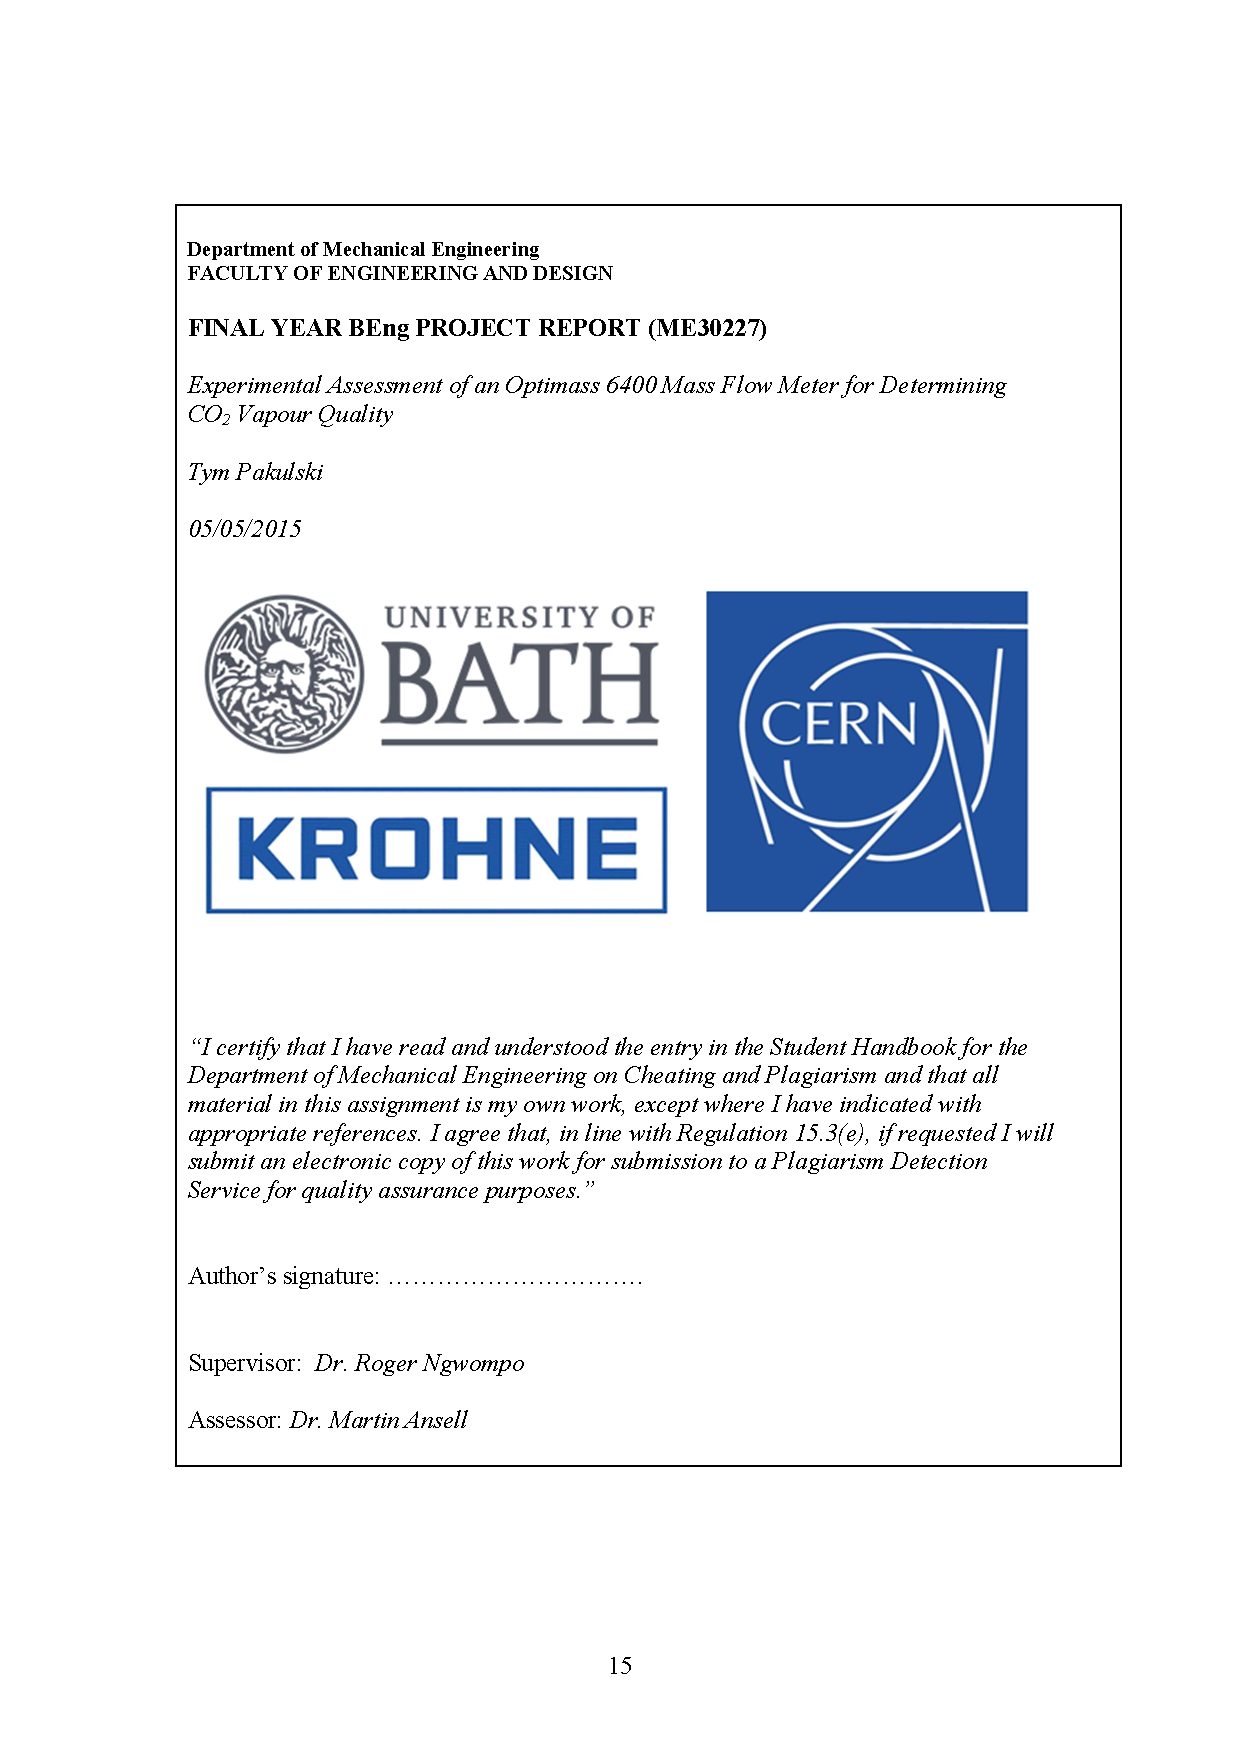
\includepdf[pages={1}]{docs/bathCoverPage.pdf}
\maketitle
\begin{abstract}
\pagenumbering{roman}
%Mention findings from lit reveiew
\end{abstract}
\section*{Acknowledgments}
Thanks to Dr. Roger Ngwompo, my academic supervisor, and Dr. Martin Ansell, FYP coordinator, for making my continued collaboration with CERN possible. I'd also like to thank Nicola Spadavecchia, Bart Verlaat and Jerome Noel for their technical support. Finally, my thanks to Paola Tropea, my industrial supervisor, for her sharp questions and crucial guidance throughout my research. 
\newpage
\section*{Terms and Acronyms}
\begin{acronym}
\acro{CERN}{The European Oranization for Nuclear Research} 
\acro{Nikhef}{National Institute for Subatomic Physics, Amserdam, Netherlands}
\acro{HEP}{High-Energy Physics}
\acro{CMS}{Compact Muon Solenoid - a CERN experiment} 
\acro{LHC}{Large Hadron Collider}
\acro{2PACL}{Two-phase accumulator control loop}
\acrodef{LS1}[sc]{Long Shutdown One}{A planned shutdown of the LHC between February 2013 and April 2015 for maintenance and upgrade.}
\acro{CFCs}{Chlorofluorocarbons} 
\acrodef{Tracker}[SC]{Type of particle detector that tracks the paths of charged particles.} 
\acro{TIF}{Tracker Integration Facility}
\acro{PH-DT}{CERN Physics Department, Detector Technologies Group}
\acro{EGM}{Entrained Gas Management}
\acro{DAQ}{Data Acquisition}
\acro{SCADA}{sc}
\acro{PWM}{Pulse Width Modulation}
\acro{R744}{Refrigerant Code for CO$_2$}
\acro{Sub-cooling}{sub}
\acro{Interaction Point}{point}
\acro{.csv}{Comma-Seperated Value}
\acro{$C_6F_{14}$}{Perflourohexane, a common industrial refrigerant and electrical insulator.}
\end{acronym}
\section*{Symbols}
\begin{center}
\begin{tabular}{|c|c|c|}
\hline
\textbf{Symbol} & \textbf{Property} & \textbf{Default Unit} \\\hline
H & Enthalpy & J \\\hline
X & Vapour Quality & \% \\\hline
T & Temperature & $^\circ$C\\\hline
$\dot{m}$ & Mass Flow Rate & kgs$^{-1}$ \\\hline
P & Pressure & bar abs \\\hline
$\dot{Q}$ & Heat Load & Watts \\\hline
$\phi$ & Void Fraction & \% \\\hline
G & Mass Flux & kgs$^{-1}$m$^{-2}$\\\hline
%thermal diffusivity
I & Current & Amperes \\\hline
V & Voltage & Volts \\\hline
p & Power & Watts \\\hline
$\rho$ & Density & kgm$^{-3}$\\\hline
v & velocity &  ms$^{-1}$\\\hline
\end{tabular}
\end{center}
\tableofcontents
\chapter{Introduction}
\pagenumbering{arabic}
\doublespacing
CERN's PH-DT group is undertaking extensive research and development in the area of evaporative CO$_2$ cooling for particle detectors. A crucial parameter in the design and commissioning of these systems is vapour quality - the mass fraction of fluid that is vapour. Krohne, a supplier of instrumentation for the process industry, has approached CERN with a new instrument with potential to indirectly determine vapour quality through a measurement of 2-phase density. This study seeks to evaluate this promising new technlogy that would be directly relevant to the coming decade of R\&\ignorespaces D. 
\section{CO\texorpdfstring{$_2$}{TEXT} Cooling at CERN}
%Background - CERN, CO2 cooling and 2PACL
The particle detectors at CERN's various experiments require cooling to manage the heat load of the detector electronics, radiation from the interaction point and heat leak from the ambient environment. Evaporative CO$_2$ cooling has become the predominant candidate technology for future particle trackers in HEP. CO$_2$'s combination of thermodynamic properties and radiation hardness make it ideal for HEP applications - it can be used in highly radioactive areas and is considered environmentally friendly. In addition, it cools efficiently in small-diameter tubes, minimising the material budget - a crucial metric representing the amount of non-instrumentation material inside the particle detector. \\The $C_6F_14$ current cooling system for the pixel detector, the innermost layer of the CMS tracker, is  being replaced with a CO$_2$ system aned a transition to this technology is foreseen for the entire CMS tracker by the end of 2024.

\begin{figure}[h!]
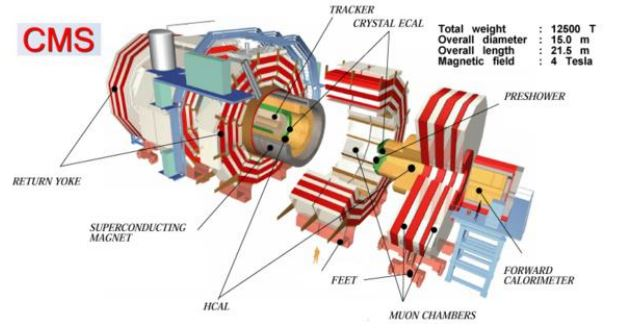
\includegraphics[width=\textwidth]{figures/CMS.jpg}
\caption{A diagram of the CMS particle detector on the LHC. \cite{mishra}}
\label{fig: cms}
\end{figure}	
\section{2-Phase Accumulator Controlled Loop}
The CO$_2$ systems at CERN implement the 2PACL design. \cite{Daguin 2012}. This involves pumping liquid coolant into the the detector, where it is expanded and cools its surroundings by partially evaporating. After cooling the detector with the latent heat of vaporisation, the mix of liquid and vapour returns to the plant by way of a condenser, which returns it to pure liquid phase for pumping. An accumulator filled with 2-phase fluid sits on the return line of the circuit, its pressure determining the position of the coolant temperature (and pressure as both are saturated), and therefore the position of the cooling cycle on the P-h diagram. Accumulator pressure is regulated using an array of heaters and a heat exchanger with an independent chiller circuit that also cools the condenser. The cycle and a schematic of the 2PACL concept are shown in figure \ref{fig:2PACL}.
\begin{figure}[h!]
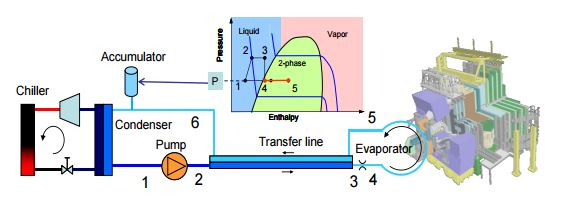
\includegraphics{2PACLschem}
\caption{A schematic of the 2PACL concept as implemented in Thermal Control System of the LHCb Velo project at CERN \cite{CO2 PoS}}
\label{fig:2PACL}
\end{figure}

\section{Vapour Quality and 2-Phase Density}
Vapour quality refers to the fraction of a fluid's mass that is in the vapour phase.
\begin{eqnarray}
X=\frac{m_{vapour}}{m_{fluid}}
\end{eqnarray}
In 2PACL cooling systems, the vapour quality after the coolant evaporates in the detector volume is an essential system parameter indicating the amount of evaporation that has occurred. The quality determines how far from the coolant is from dry-out, where a dramatic decrease in heat transfer coefficients may occur, causing a sudden decrease in cooling. A real-time calculation of vapour quality would allow the design of leaner cooling systems as dry out conditions can be observed before they occur, reducing the safety factors taken in sizing the liquid mass of the system.\\
Vapour quality at any point on a P-h diagram can be determined using the lever rule inside the vapour dome. In 2PACL, the challenge is mapping the fluid's exact location. In pure liquid, any point on the P-h diagram can be determined from pressure and temperature, but in phase transition these values are saturation conditions, and therefore a third variable is needed. One obvious choice is density, as shown in Figure \ref{fig:densityMethod}. By knowing the local pressure and density, the exact point in the vapour dome, and therefore the vapour quality, can be determined. 

\begin{figure}
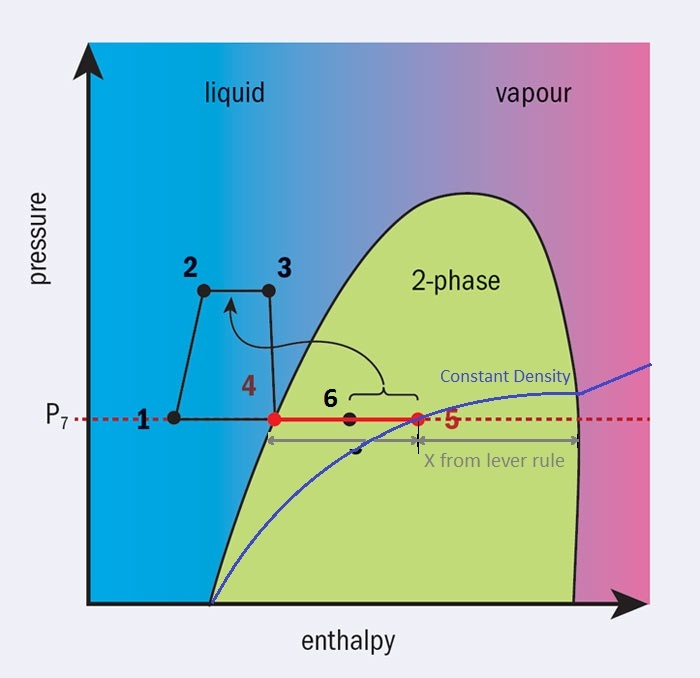
\includegraphics[width=0.5\textwidth]{densityMethod.jpg}
\caption{Principle for determining vapour quality, \textit{X}, from two-phase density. Adapted from B. Verlaat. \cite{CERN courier}}
\label{fig:densityMethod}
\end{figure}

\section{The Krohne Optimass 6400}
The Optimass 6400 is a new twin bent tube coriolis mass flow meter. It features 3 independent measurements, from which it calculates 7 output signals. The 3 fundamental measurements to be assessed are:
\begin{itemize}
\item{Mass Flow Rate - Coriolis principle.}
\item{Density - Natural frequency of an oscillating tube.}
\item{Temperature - Internal probe.}
\end{itemize}
\begin{figure}
\includegraphics[width=0.4\textwidth]{Optimass6400}
\caption{The Krohne Optimass 6400 mass flow meter.} %cite KROHNE DATA SHEET}
\label{fig:optimass6400}
\end{figure}
The instrument is unique because of its Entrained Gas Management - it is able to continue reading mass flow, density and temperature of 2-phase flow. The instrument's accuracy has been measured using liquid water and air bubbles, but never with a single fluid in 2 phases. 
\section{Aims, Objectives and Documentation}
This study is an initial evaluation of the Optimass 6400's steady-state measurement accuracy over a wide operating envelope. Its aim is to evaluate the validate the strategy for determining vapour quality, quantify the attainable measurement under various conditions, and identify performance trends and areas for further research. Specific goals are given below:
\begin{itemize}
\item{Compare mass flow and density readings with reference instrumentation and theory over a range of temperatures and vapour qualities.}
\item{Quantify the instrument's steady-state performance and, if possible, identify an effective performance envelope.}
\item{Express the instrument's accuracy in terms of vapour quality.}
\item{Investigate the physical phenomena behind any performance trends.}
\item{Identify areas for further research.}
\end{itemize}
This report documents the background to the problem and relevant literature, describes the method employed to test and analyse the sensor's performance in \ref{methods}, and the results of the testing in \ref{results}. Further, it documents speculation as to the cause of performance trends revealed in \ref{results} and identifies areas for further research in \ref{further research}.


\chapter{Literature Review}
\section{Behaviour of 2-Phase CO$_2$}
%Flow mapping
%dry out and HTCs
%reduced pressure

\section{Determining Vapour Quality}
Literature on direct measurement of vapour quality is scarce, especially for CO$_2$. B.R. Jean presented a steam quality sensor that employs microwaves, yielding an accuracy of 2.8\%. \cite{Jean 2007}. The operating principle relied on the dielectric properties of water. A review of steam quality measurement approaches conducted by Dorman and Fridman \cite{Dorfman 2006} evaluated calorimeter, chemical tracer and flow seperation methods, revealing their significant drawbacks. The authors then presented a new theoretical method for measuring vapour fraction, but it was limited to fluid in a static container. \\
Void fraction, defined as the volumetric fraction of fluid in the vapour phase, is an intuitive candidate for an inderect measurement of vapour quality. 
\begin{eqnarray}
\phi =\frac{V_{vapour}}{V_{fluid}}
\end{eqnarray}\\
Indeed, several methods have been developed for the measurement of void fraction, relying on capacitance measurement \cite{Beker 2005}, x-rays \cite{Bauer 2012}, electron sources \cite{Augyrond 2001} and gamma ray densiometers \cite{Zhao 2013}. However, the conversion of void fraction to vapour quality is far from straightforward, as the mass fraction of vapour depends on the density of both the vapour and the fluid:
\begin{eqnarray}
X =\phi\frac{\rho_{vapour}}{\rho_{fluid}}
\end{eqnarray}
Emperical relations have been developed, most notably by Zuber and Findaly, between void fraction and vapour quality, but their complexity and limited range makes them impractical for a real-time application.\cite{lecture}.

%analytical methods
\section{Measuring 2-Phase Density}
\section{Coriolis Flow Meters' Performance in 2-Phase}
Coriolis flow meters induce a phase shift in the forced oscillations of two bent tubes using the Coriolis principle. As the tubes vibrate at their natural frequency, the velocity of the flow as it is directed radially toward and away from the axis of oscillation in the bent sections induces a phase shift varying linearly with the mass flow rate of the fluid through the instrument. \cite{O'Banion 2013} A schematic of the principle is given in figure \ref{fig:coriolis}. \\
\begin{figure}
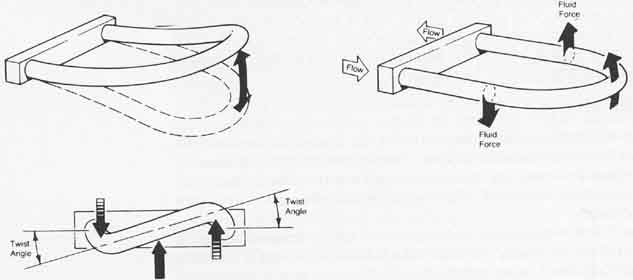
\includegraphics[width=0.6\textwidth]{coriolis}
\caption{The working principle of coriolis flow meters. \cite{coriolis}}%find this reference
\label{fig:coriolis}
\end{figure}
Density, when independently measured in coriolis flow meters, is typically determined from the resonant frequency of the bent tubes. \cite{O'Banion 2013} The frequency is a function of the tube stiffness and mass. So any change in mass reflects a change in density of the fluid insisde the tube. The sensor corrects for temperature effects on stiffness and, with a known tube volume, determines the density.\\
Both of these measurement principles can be severely disrupted by 2-phase flow. Entrained gas may create slip planes between the phases, which cause unpredictable forces and vibrations.\cite{ISO}\cite{processArticle} This leads to two problems in instrumentation: first, the unexpected vibrations disturb sensitive electronics. Second, the slip between the phases dampens forced vibrations, possibly stopping the sensor from reading altogether. In a typical coriolis flow meter, the first symptom of entrained gas is the drive gain, the power required to force the tubes' oscillation, rising to 100\%. \cite{ISO}\cite{emerson youtube}\\
Some manufacturers of process instrumentation have developed products to detect entrained gas. The Emerson Rosemount 3051S Pressure Transmitter, for example, employs statistical methods to detect characteristic frequencies of entrained gas.\ref{emerson EGM}\\
%2-phase flow meter performance lit review




The Optimass 6400 is a physical copy of the older Otpimass 6000. But what makes it unique is the MFC400 electronics chip that it interfaces with. These electronics deliver Entrained Gas Management. A typical flow meter cannot handle 2-phase flow because the slip planes between the liquid and vapour phases damp the oscillations, causing the instrument to stop reading. Entrained Gas Management employs advanced signal processing and a completely digital drive signal to allow the instrument to continue measuring in 2-phase flow. \cite{krohne brochure}\cite{processArticle}\\



\chapter{Methods} \label{methods}
\section{Experimental Methods}
Laboratory research was carried out using the future CMS pixel detector cooling system located in the Tracker Integration Facility clean room at CERN. This cooling system, hereafter referred to as \textit{TIF}, employs the \textit{2PACL} concept for evaporative CO$_2$ cooling. It allows active control of the coolant temperature, its flow rate and the heat load applied to  it. \\
\textit{TIF} consists of a membrane pump routing liquid CO$_2$ through a concentric transfer line to a manifold where the flow is split and can be heated. \textit{Dummy Load} heaters represent the detector heat load, evaporating the CO$_2$ in the manifold. An accumulator containing 2-phase fluid on the return line of the manifold regulates the pressure set point using an array of heaters and a heat exchanger. A freon chiller cools the accumulator and the condenser at the pump inlet.\\
A full Process and Instrumenation Diagram is given in Appendix \ref{appTIF}.
\subsection{Apparatus}
%The TIF room and the future pixel cooling system
%appendix: TIF P & I
%plant configuration
%ADD INSTRUMENT INITIALLY VALIDATED IN LIQUID FLOW

\begin{figure}
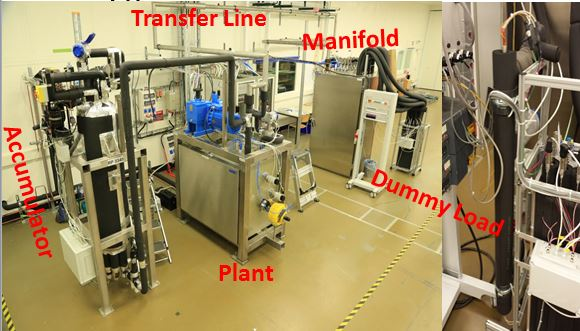
\includegraphics[width=\textwidth]{TIFandHeater.jpg}[h!]
\caption{The TIF cooling plant[L] and dummy load heater [R]. \cite{tif web}}
\label{fig:TIF}
\end{figure}

The TIF cooling system services 8 cooling loops in the manifold and includes several bypasses, heaters and instrumentation that are mostly relevant to the  start-up procedure and are configured using a series of pneumatic, manual and electro-mechanical valves. 
The plant was configured the same way for all tests: with all bypass loops closed, and a single loop, number 7424, open in the manifold. This configuration ensured all fluid leaving the plant passed through this loop and the Optimass instrument, and allows the experimental apparatus to be represented by a simplified P \& I diagram given in figure \ref{fig:TIFsimplified}.
\begin{figure}
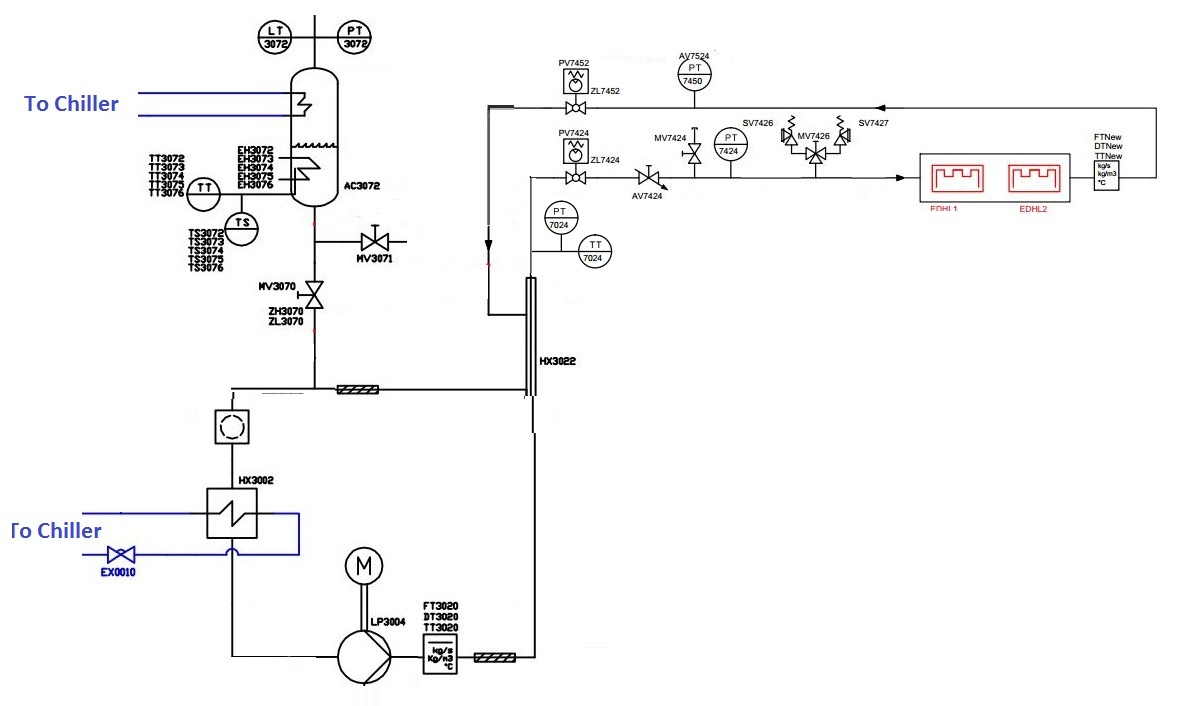
\includegraphics[width=\textwidth]{TIFsimplified.jpg}
\caption{A simplified process and instrumentation diagram of the TIF cooling plant in the configuration relevant to the tests, displaying only relevant instrumentation. A diagram of the whole TIF if given in appendix \ref{app:TIF}}
\label{fig:Tifsimplified}
\end{figure}

%instrument physical mounting
The Optimass instrument was mounted on a test stand close to the \textit{TIF} manifold, as shown in figure \ref{fig:sensor}. Following guidance from Krohne, it was mounted upside-down, with the electronics module closer to the floor. The instrument's discharge was connected through a flexible pipe to the the return lines of loop 7424 in the \textit{TIF} manifold. On the supply side, the instrument was connected directly to the discharge of the heating section. 
\begin{figure}
        \centering
        \begin{subfigure}[b]{0.5\textwidth}
                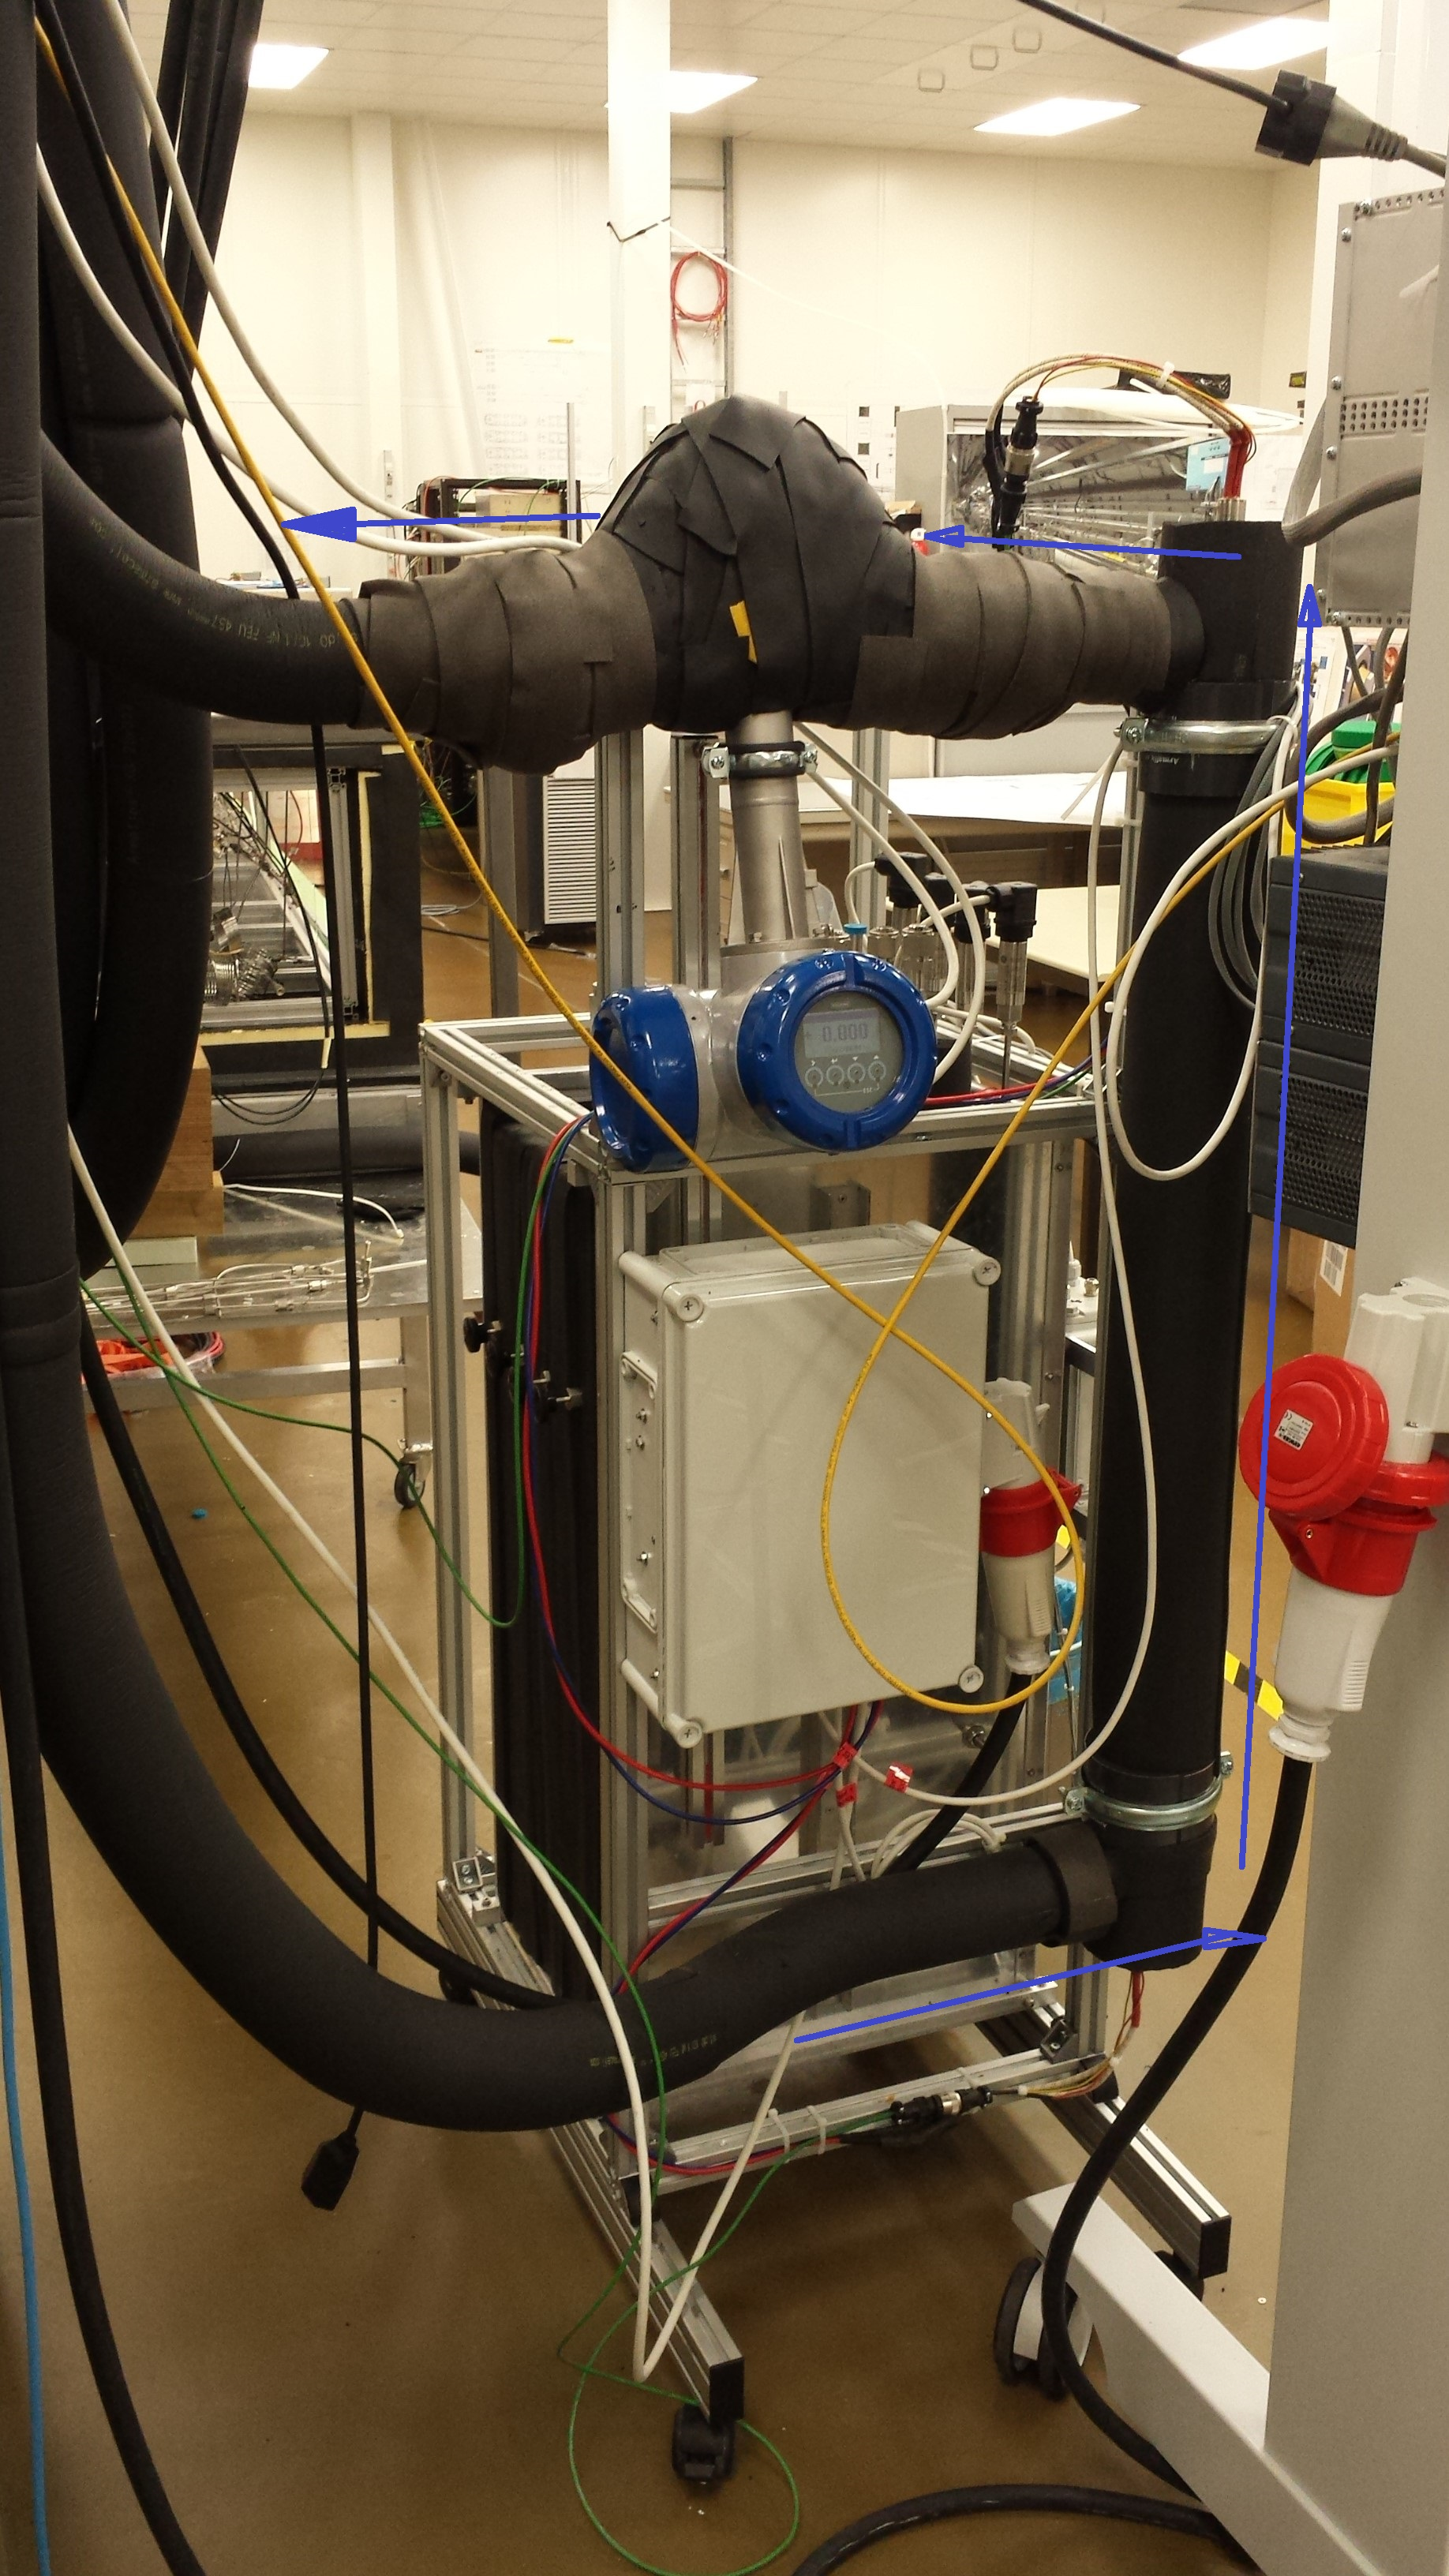
\includegraphics[width=\textwidth]{sensor}
                \caption{Front view.}
  				\label{fig:sensor}
        \end{subfigure}%
        ~
        \begin{subfigure}[b]{0.5\textwidth}
                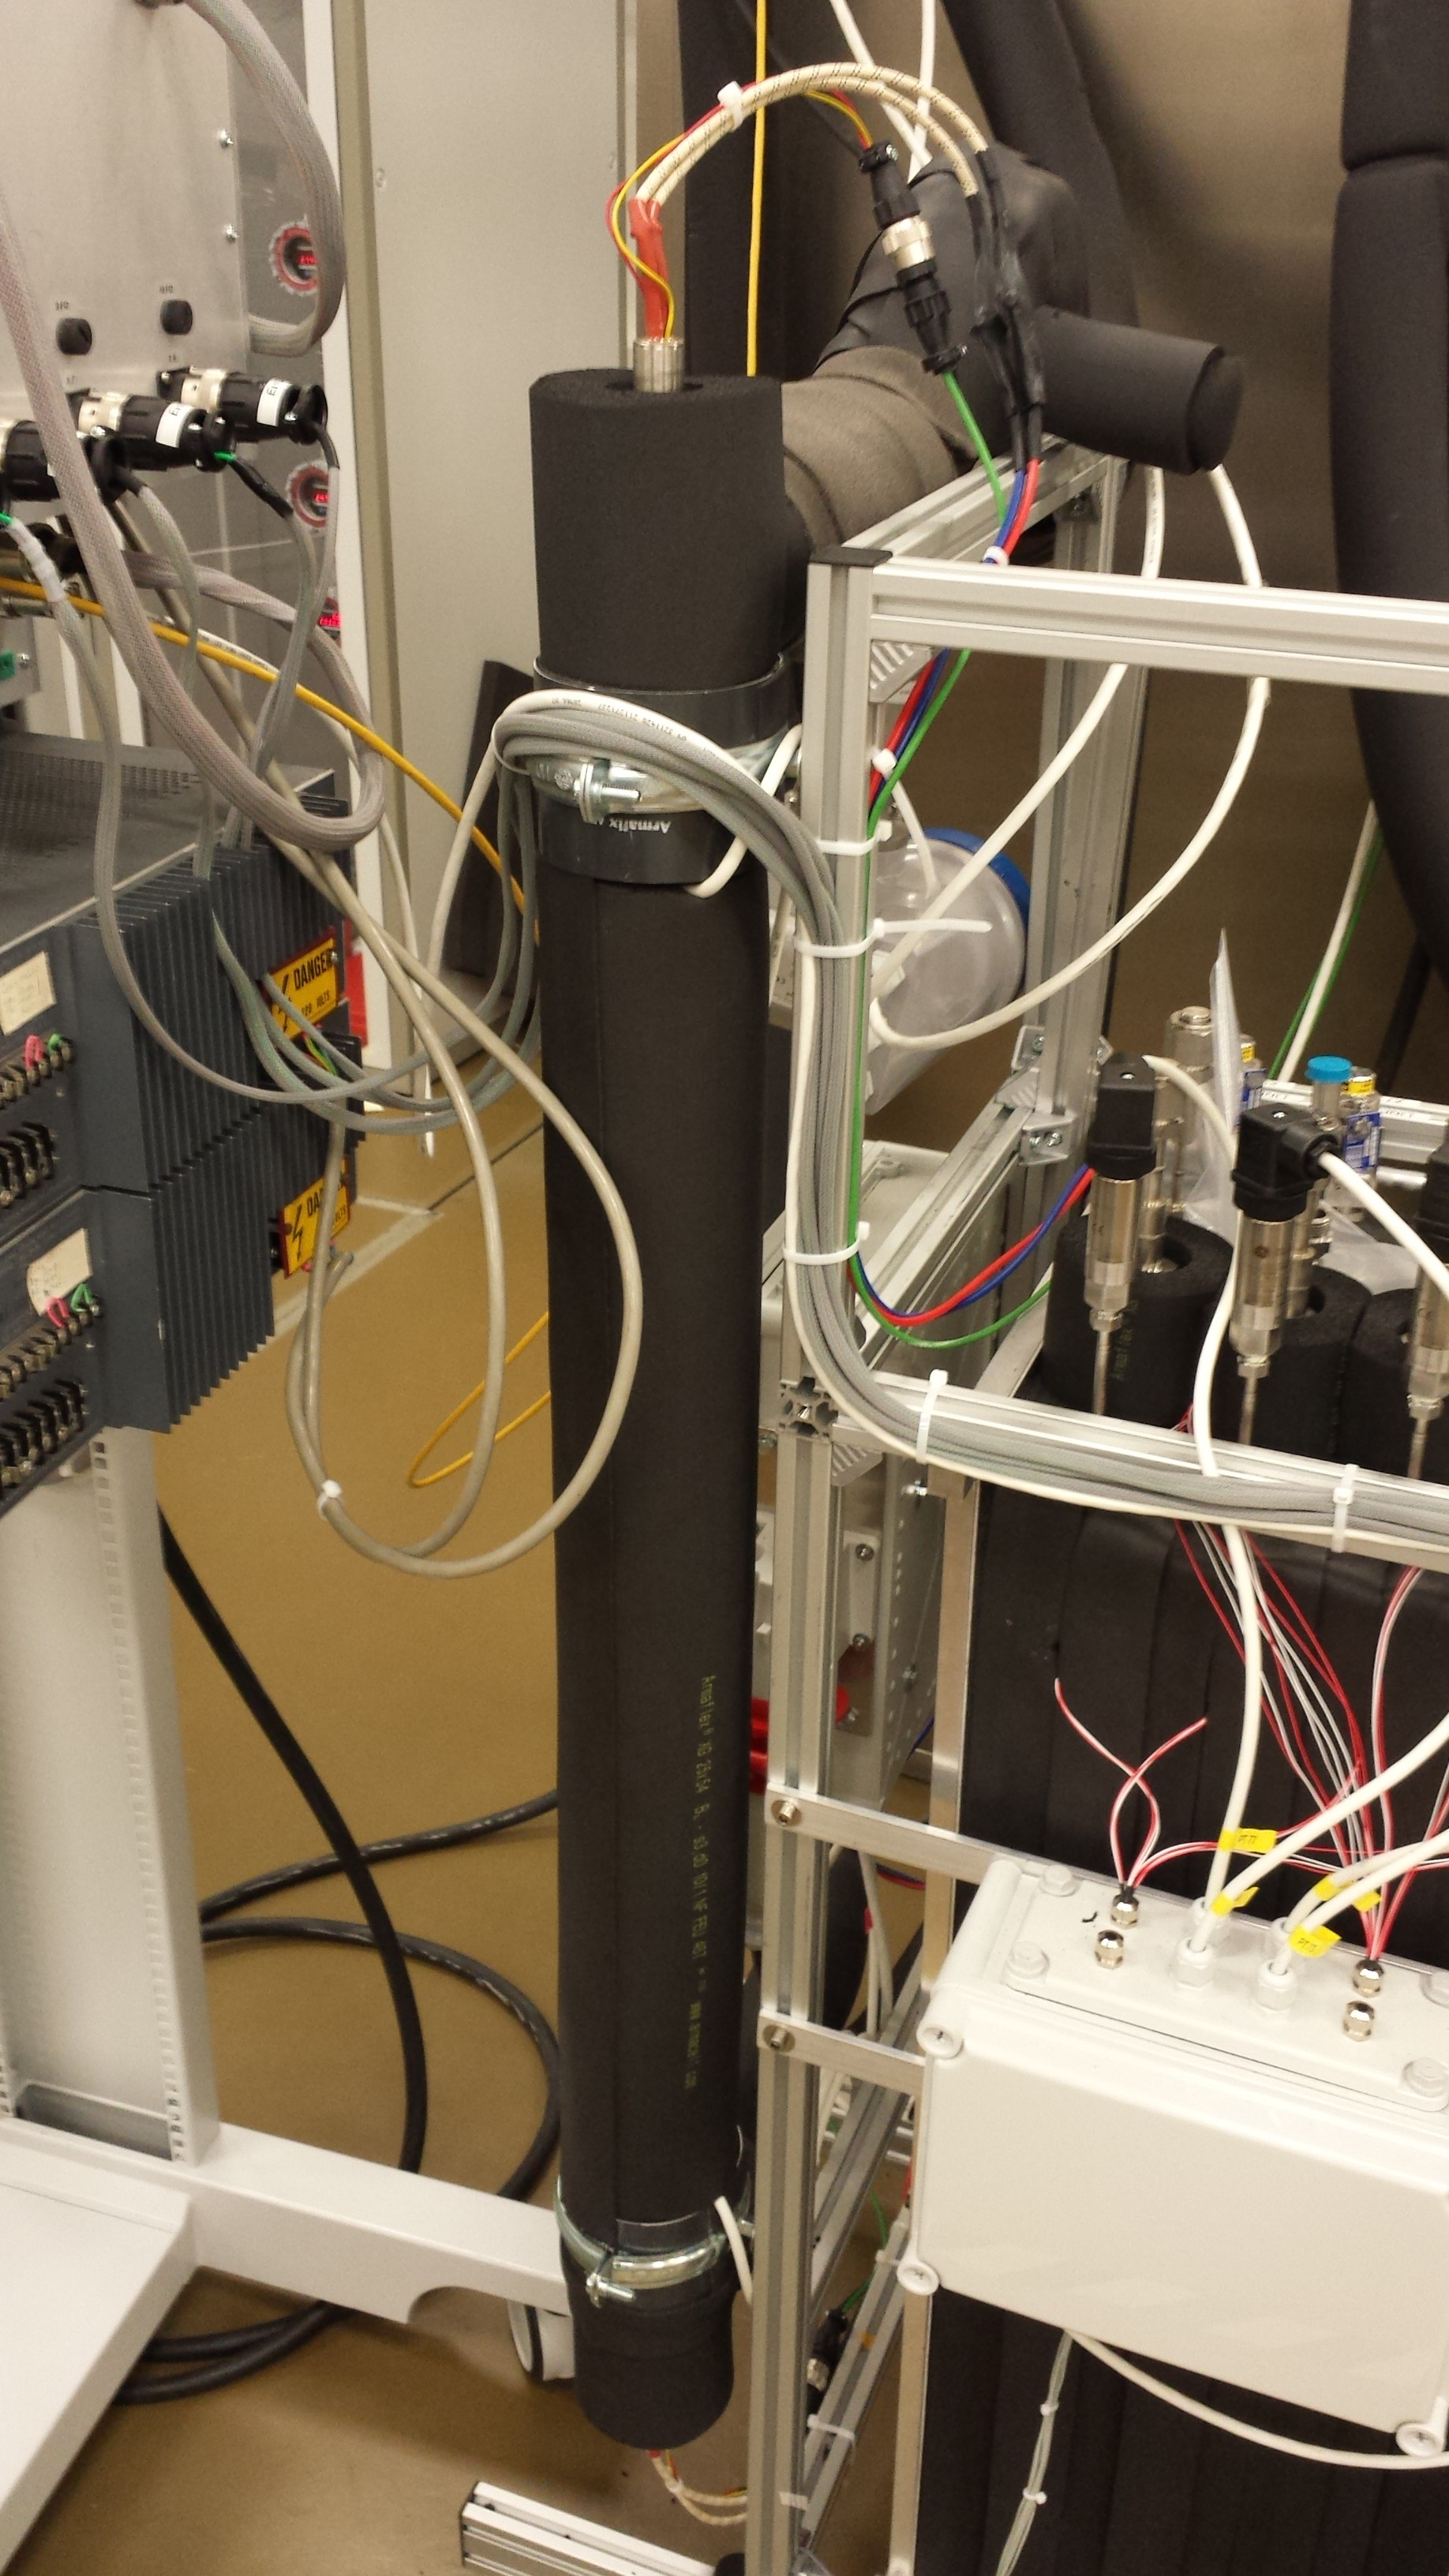
\includegraphics[width=\textwidth]{heaterCloseUp}
                \caption{Side view.}
  				\label{fig:heaters}
        \end{subfigure}
        ~ %add desired spacing between images, e. g. ~, \quad, \qquad, \hfill etc.
          %(or a blank line to force the subfigure onto a new line)
          \caption{Photographs of the Optimass sensor connected to the dummy load heating section. The direction of flow is given by the blue arrows.}
\end{figure}
%heating section 
The heating section of loop 7424 consists of a 35 mm OD vertical pipe welded to two tee unions. Two cartridge heater inside 22 mm pipes are axially inserted into the pipe through the tee fittings, as shown in figure \ref{fig:heaters}. A drawing of the heater is given in Appendix \ref{app:DummyLoad}. The flow enters the heating section radially with respect to the heaters through the lower tee union. It is forced into an anuular shape encircling the heater, and flows upward to the discharge tee-union. It then enters a short unobstructed circular series of fittings before reaching the Optimass instrument. Guidance from Krohne engineers and the instrument documentation indicated that the geometry at the sensor in let was satisfactory.
%insulation
The vacuum-insulated instrument, as well as all exposed piping, was covered with a 20 mm layer of \textit{Armaflex} insulation to mitigate heat pick-up. All fittings were leak tested at 50 bar gas using a CO$_2$ sniffer prior to testing, and the instrument's position and inlet conditions respected the guidelines given in Appendix, as well as input from Krohne engineers. 

%Simplified P & I
%Operational Envelope 
\subsection{Control and Data Acquisition}
All of the instrumentation on the TIF plant, the dummy load and the Optimass flow meter is cabled to a central PLC in the TIF clean room. Each instrument communicates a 4-20 mA analogue current signal, which is mapped by the PLC to produce a value in the correct units. All of the data is continuously logged to a server, day and night. The data is logged using a change or duration algorithm - logging new data only when one of the signals has changed. This produces a sampling rate of several Hz during transient conditions - meaning hundreds of thousands of data points over the 3-week test campaign.
The Optimass sensor was configured by Krohne Italy to deliver mass flow, density and temperature signals through a 4-20 mA bus in the following measurement ranges:\\
\begin{itemize}
\item{Mass Flow Rate: 1.4-115 g/s} %check this
\item{Density: 100.6 - 1200 $kgm^{-3}$}% is it?
\item{Temperature: ????}
\end{itemize}
The sensor was cabled to the same PLC controlling TIF and logging all of its instrumentation, and the signals were mapped to the values configured by Krohne. This approach streamlined control and post-processing by consolidating the plant, heaters and instrument on a single Scada interface, and logging the data in a single location at common timesteps. 
\subsection{Variables and Assumptions}
The instrument's performance was to be assessed in relation to three independent variables:
\begin{itemize}
\item{Coolant temperature - regulated by the accumulator set point.}
\item{Mass flow rate - set by the pump speed and stroke.} 
\item{Heat Load - set by the heaters' rms current.}
\end{itemize}
The coolant temperature set point determines the position along the vapour dome on a P-h diagram of the 2PACL cycle, and therefore the local pressure in the instrument. This influences the evaporative behaviour of the coolant, as well as the vapour quality for a given density. While a wide range of temperature was to be explored, the invariance of the temperature during a tests was an essential control variable. \\
The mass flow rate was set by the speed and stroke of the pump, but not regulated during tests. This meant that as the vapour quality of the coolant increased, the resultant increase in pressure drop decreased the effective flow rate for given pump conditions. The resulting fluctuations in true flow rate affect the trends plotted by nominal flow rate, but because flow rate is measured in real time, they did not effect error signal calculations.\\
The dummy load heaters are resistive cartridge heaters, whose power is controlled by pulse width modulation. The user specifies a Watt value on the Scada interface, and the PLC applies the correct PWM signal to achieve the demand power output. Heater control is open-loop, but their performance has been validated in the past. %????
\\
A broad range of all three variables was explored. But because this experiment sought only to evaluate steady-state performance, transient data was to be minimised. The control variables were therefore closely monitored to minimise fluctuations. 
\subsection{Test Protocol}
Before beginning 2-phase testing, the instrument's calibration was validated in pure liquid by comparing its readings of mass flow, density and temperature with a reference instrument on the plant (FT3020) for a range of flow rates and temperatures.\\
For 2-phase testing, a test protocol was developed to ensure consistency of data. A change to any of the independent variables caused a significant transient response. But the process of fine-tuning the values and waiting for their response to settle differed for each variable. Tests were designed accordingly.\\\\
\begin{center}
\begin{table}
\begin{tabular}{|l|l|l|l|}
\hline
\multicolumn{3}{ |c| }{\textbf{Key Variables and Settling Times}} \\\hline
\textbf{Variable} & \textbf{Control Method} & \textbf{Settling Time}\\\hline
Temperature & Accumulator Set Point & 30-90 minutes\\\hline
Mass Flow Rate & Pump speed and stroke & 15-30 minutes\\\hline
Vapour Quality & Dummy Load Power & 5-15 minutes\\\hline
\end{tabular}
\caption{Key variables, their control method and their settling times.}
\label{tab:settle}
\end{table}
\end{center}
Altering test conditions employed a nested approach. First, the coolant temperature was set in the accumulator. Then various heat loads were applied at a given pump speed to explore a range of vapour qualities at a given flow rate, before changing the pump conditions. A typical test segment: various heat loads at a given flow rate and temperature, is shown in Figure \ref{fig:typicalTest}. 

\begin{figure}
%EDIT THIS PICTURE FOR CONSTANT TEMPERATURE
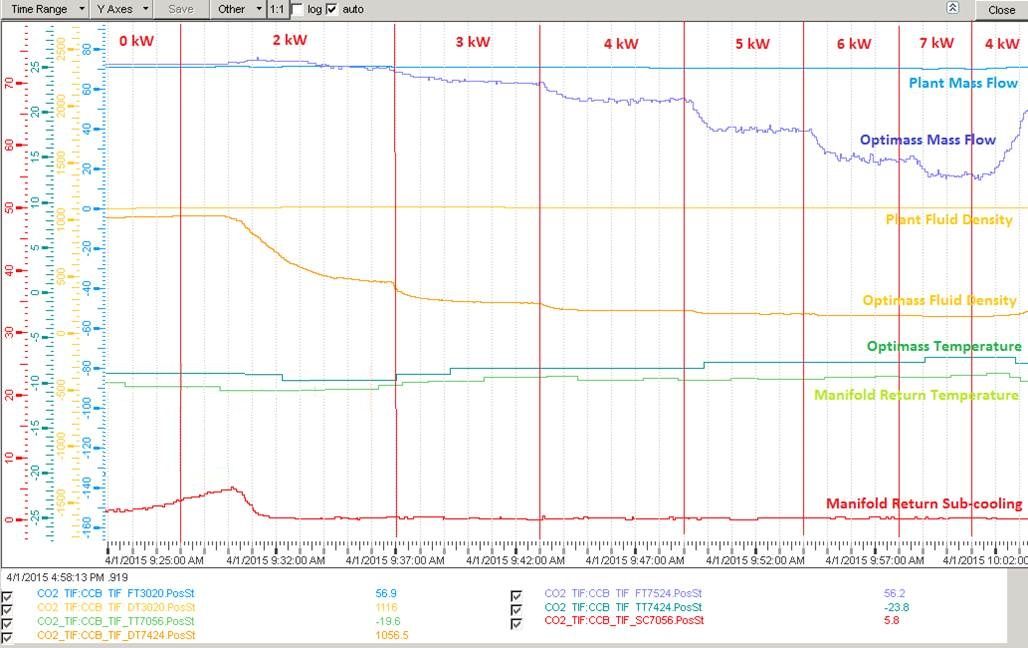
\includegraphics[width=\textwidth]{typicalTestEdited}
\caption{A typical test. The steps in heat load are shown as vertical red lines.}
\label{fig:typicalTest}
\end{figure}

\section{Data Analysis Methods}
A method, summarised in Figure \ref{fig:processing}, was devised for the export, pre-processing and process of data. This approach filtered through the hundreds of thousands of data points to reach a small subset of steady-state data during test conditions. 

\begin{figure}
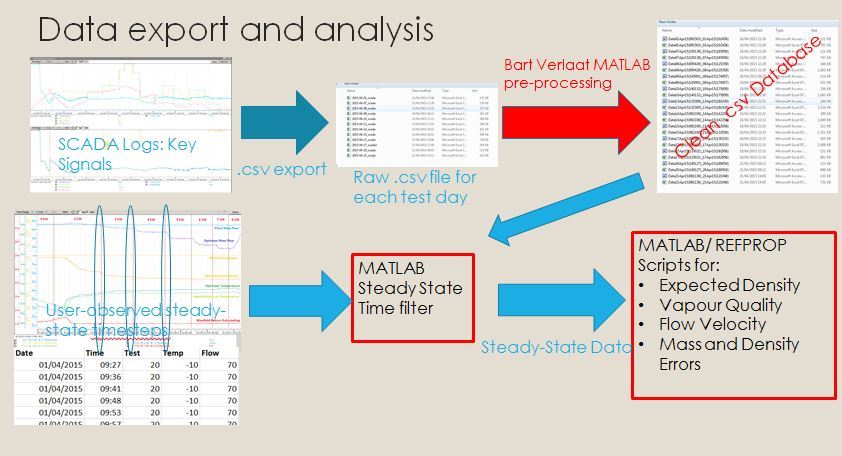
\includegraphics[width=\textwidth]{processing}
\caption{A summary of data processing and analysis.}
\label{fig:processing}
\end{figure}

\subsection{Export Pre-Processing} %database management, steady-state filtering
Including time, 12 signals out of the dozens logged in the PLC were identified as being key for this study. These are summarised in table \ref{tab:keySignals}.\\
\begin{center}
\begin{table}
\begin{tabular}{ |c|c|c|l| }
\hline
\multicolumn{4}{ |c| }{\textbf{Key Signals}}\\\hline
\textbf{Signal Type} & \textbf{Signal Name} & \textbf{Thermodynamic Symbol} & \textbf{Description} \\\hline
\multirow{3}{*}{Optimass} & FT7524 & $\dot{m}$ & Mass flow rate measured by Optimass 6400\\\hline
& DT7424 & $\rho_5$ & Density measured by Optimass 6400 \\\hline
& TT7424 & T$_5$ & Temerature measured by Optimass 6400 \\\hline
Reference & FT3020 &  $\dot{m}_{ref}$ & Liquid mass flow rate measured in plant. \\\hline
Reference & PT7024 & P$_3$ & Manifold supply pressure. \\\hline
Reference & TT7024 & T$_3$ & Manifold supply temperature. \\\hline
Reference & EHDL1 & $\dot{Q}_a$ & Dummy load heater 1 power. \\\hline
Reference & EHDL2 & $\dot{Q}_b$ & Dummy load heater 2 power. \\\hline
Reference & PT7450 & $P_5'$ & Pressure at instrument discharge. \\\hline
\end{tabular}
\caption{Key Signals}
\label{tab:keySignals} 
\end{table}
\end{center}
A page of plots tracking these signals was created in the Scada interface. Then, \textit{.csv} data for each signal was exported by navigating to the time of a given test and exporting a 4 hour window of data. These \textit{.csv} files for each day of testing were then pre-processed using modified MATLAB scripts developed by Bart Verlaat. Pre-processing involved merging the data from each test into a single database, handling empty cells and overlapping timesteps, and saving the cleaned data in a new database to be called by MATLAB. 
\subsection{Data Processing and Visualisation}
With the key signals filtered to leave only steady state conditions, these were processed to assess the sensor's performance. The sensor was evaluated by comparing its readings to a combination of reference instrumentation and analytically computed reference conditions. \\
%REFPROP mentioned here
Analysis employed an theoretical MATLAB model to compute thermodynamic state variables in the sensor, and called a refrigerant simulation program called REFPROP to compute the local conditions of interest. %refrigerant simulation??\\
REFPROP, developed by National Instruments, is a widely used program that simulates refrigerant performance using a combination of analytical and empirical methods. %true??
\subsection{Calculation of Reference Conditions}
The local density and vapour quality in the Optimass sensor are calculated using the local pressure and specific enthalpy. 
%juxtapose pure liquid and 2-phase approaches to determining position in P-h
A pressure and an enthalpy give the fluid's exact location in the vapour dome, and the vapour quality and density can be read from the chart, as shown in Figure \ref{enthalpyMethod}. This is implemented using REFPROP. With the following syntax: \\\\
\textit{Q = refpropm('Q','P',$<P_5$ [kPa]$>$ , 'H', $<h_5$ [J/kg]$>$ , 'CO2')} \\\\
The local enthalpy at the sensor, \textit{$h_5$}, is given by the sum of the manifold inlet enthalpy, $h_3$ and the change in enthalpy due to the heat load, $\Delta$h.\\
\textit{$h_3$} is determined with REFPROP from the inlet manifold inlet conditions (Pressure and Temperature in pure liquid), while the change in enthalpy is calculated from the heat load and reference mass flow rate.\\\\
\textit{$h_3$=refpropm('H','P',$<P_3$ [kPa]$>$ ,'T', $<T_3$ [K]$>$, 'CO2')}\\\\
p = Heat Load [W]\\
\begin{eqnarray}
\Delta h=\frac{p}{\dot{m}}
\end{eqnarray}
\begin{figure}
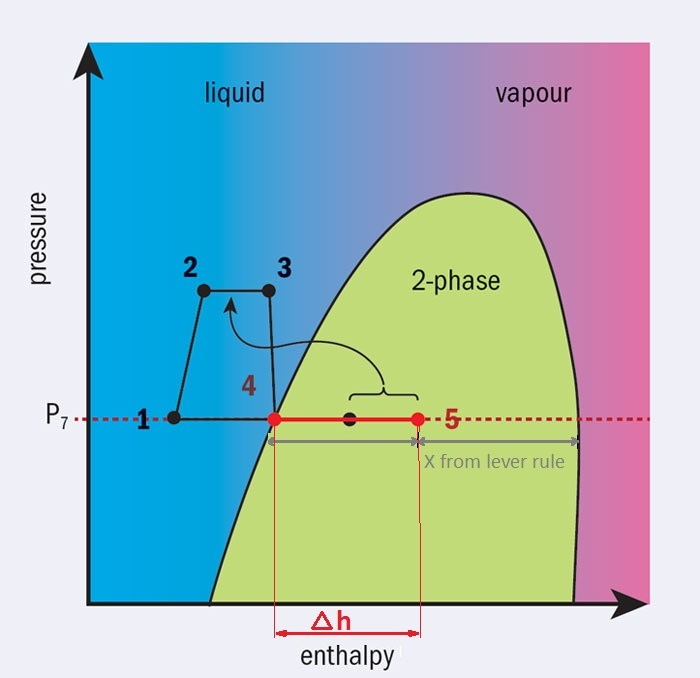
\includegraphics[width=0.5\textwidth]{enthalpyMethod.jpg}
\caption{The analytic model for calculating local 2-phase conditions at the flow meter.}
\label{fig:enthalpyMethod}
\end{figure}
\chapter{Results} \label{results}
%OVERVIEW - 2 plots 
\begin{figure}
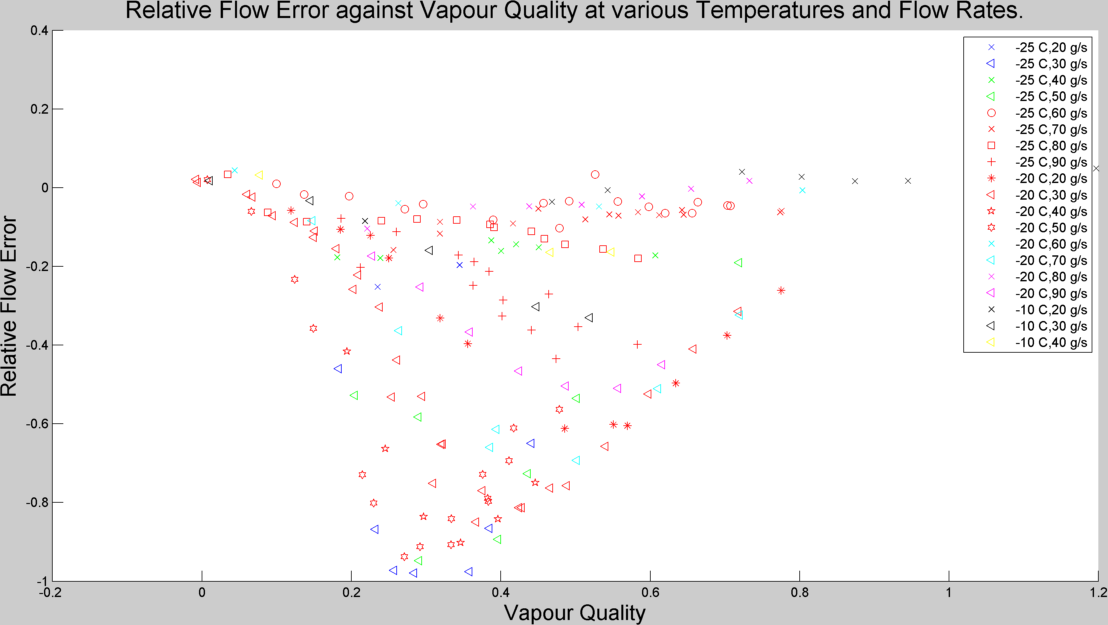
\includegraphics[width=\textwidth]{plots/fig1}
\caption{An overview of relative mass flow error against vapour quality.}
\label{plot:1}
\end{figure}
\begin{figure}
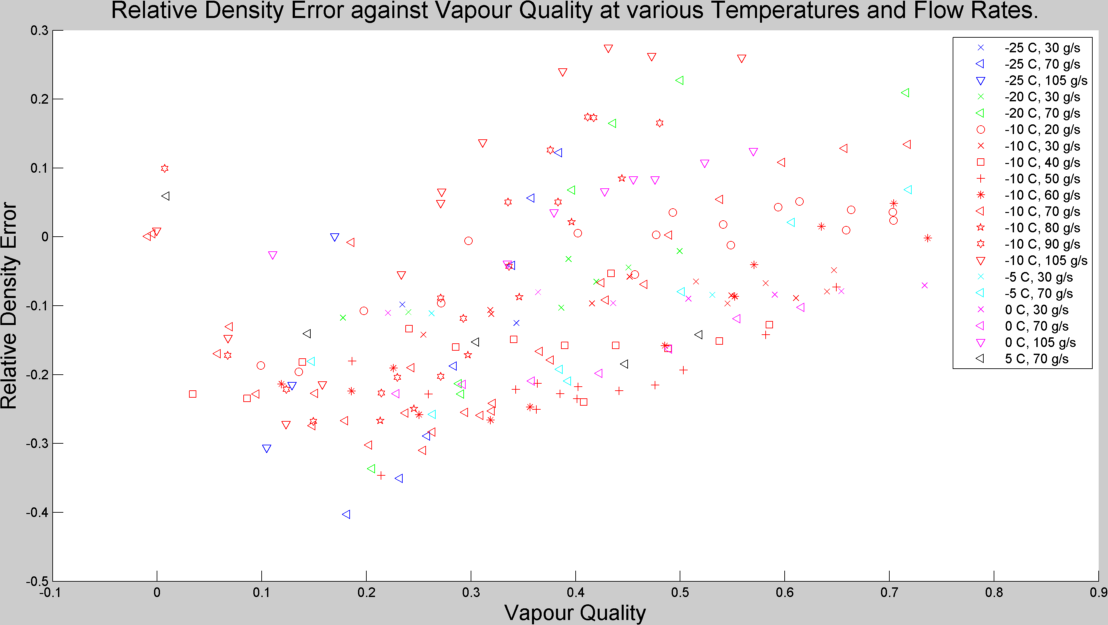
\includegraphics[width=\textwidth]{plots/fig2}
\caption{An overview of relative density error against vapour quality.}
\label{plot:2}
\end{figure}

%INTERESTING TRENDS
%MASS FLOW TREND

\begin{figure}
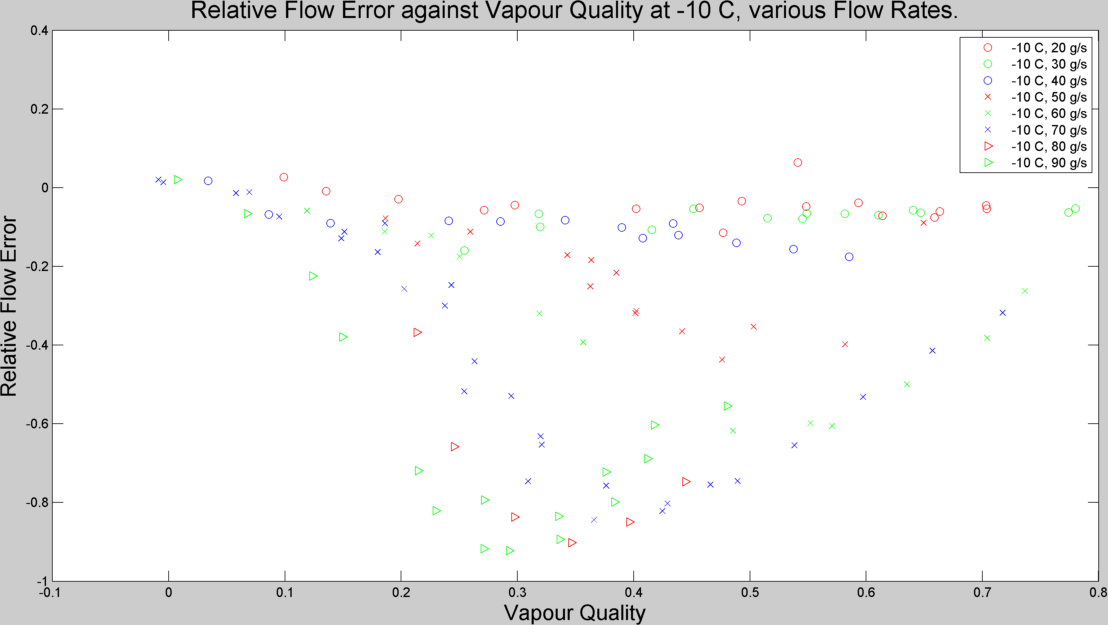
\includegraphics[width=\textwidth]{plots/fig3}
\caption{An overview of relative density error against vapour quality.}
\label{plot:3}
\end{figure}

\begin{figure}
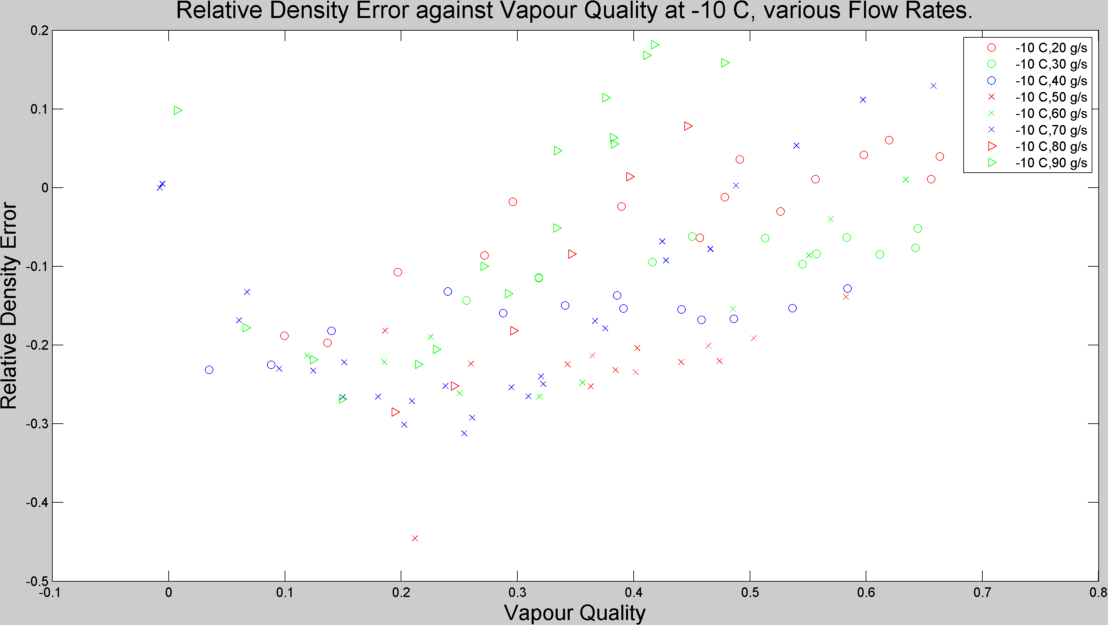
\includegraphics[width=\textwidth]{plots/fig4}
\caption{An overview of relative density error against vapour quality.}
\label{plot:4}
\end{figure}

%Temperature TREND***********************
\begin{figure}
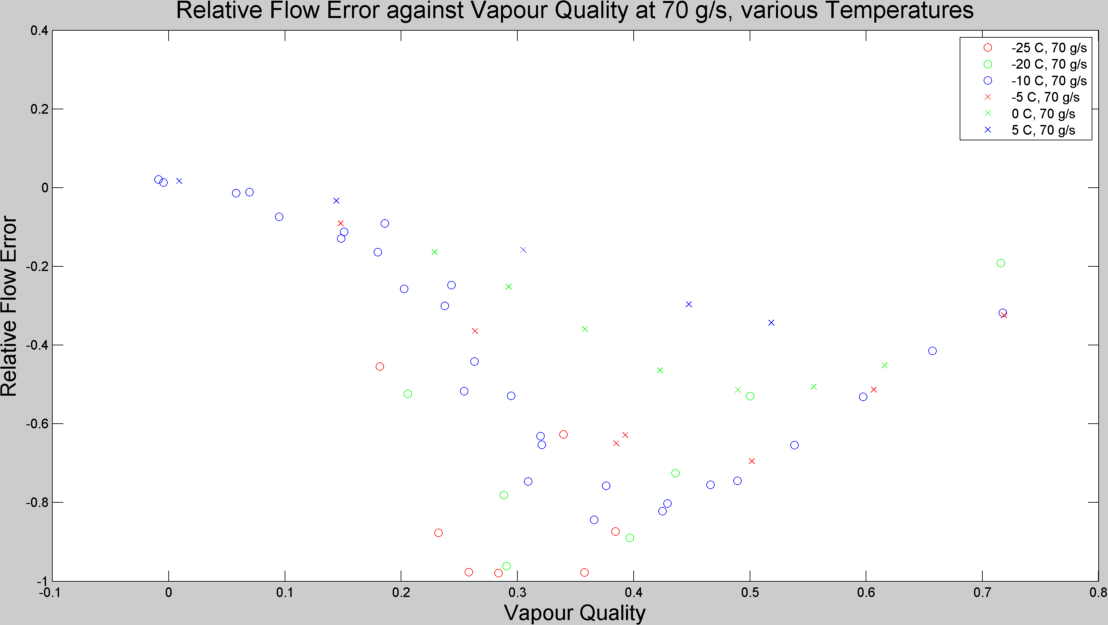
\includegraphics[width=\textwidth]{plots/fig5}
\caption{An overview of relative density error against vapour quality.}
\label{plot:5}
\end{figure}

\begin{figure}
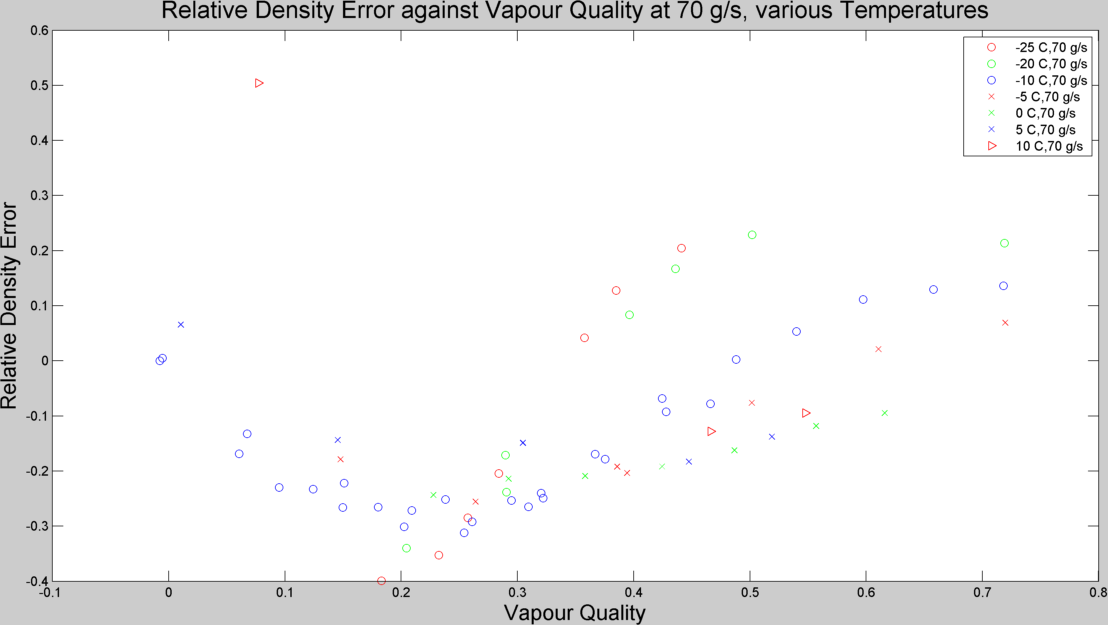
\includegraphics[width=\textwidth]{plots/fig6}
\caption{An overview of relative density error against vapour quality.}
\label{plot:6}
\end{figure}

%time responses typical
%two interesting trends
\begin{figure}
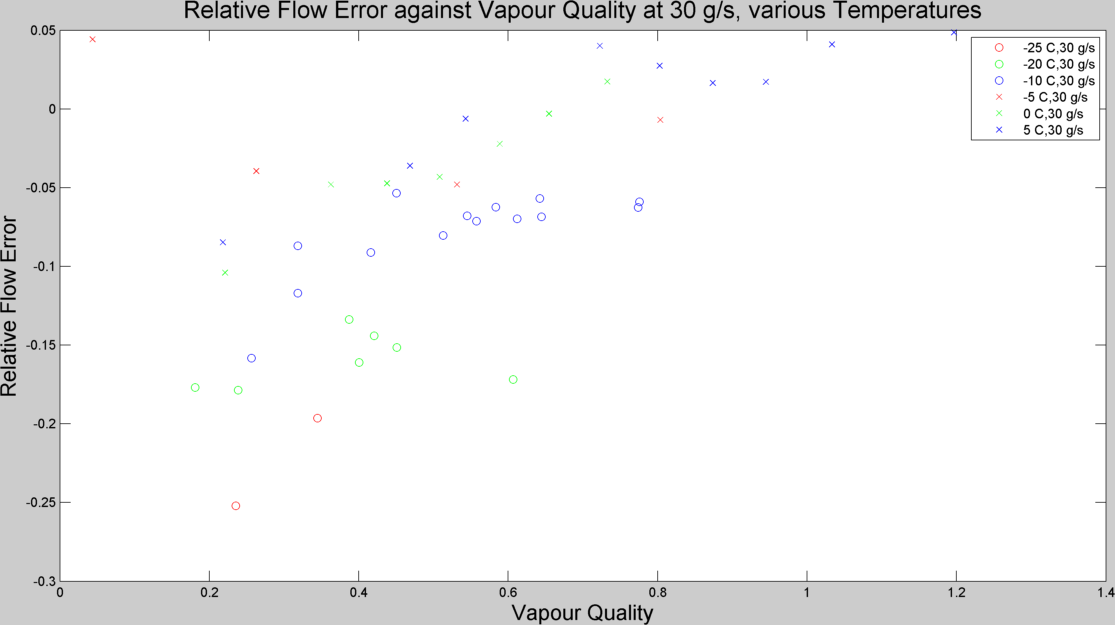
\includegraphics[width=\textwidth]{plots/fig7}
\caption{An overview of relative density error against vapour quality.}
\label{plot:7}
\end{figure}

\begin{figure}
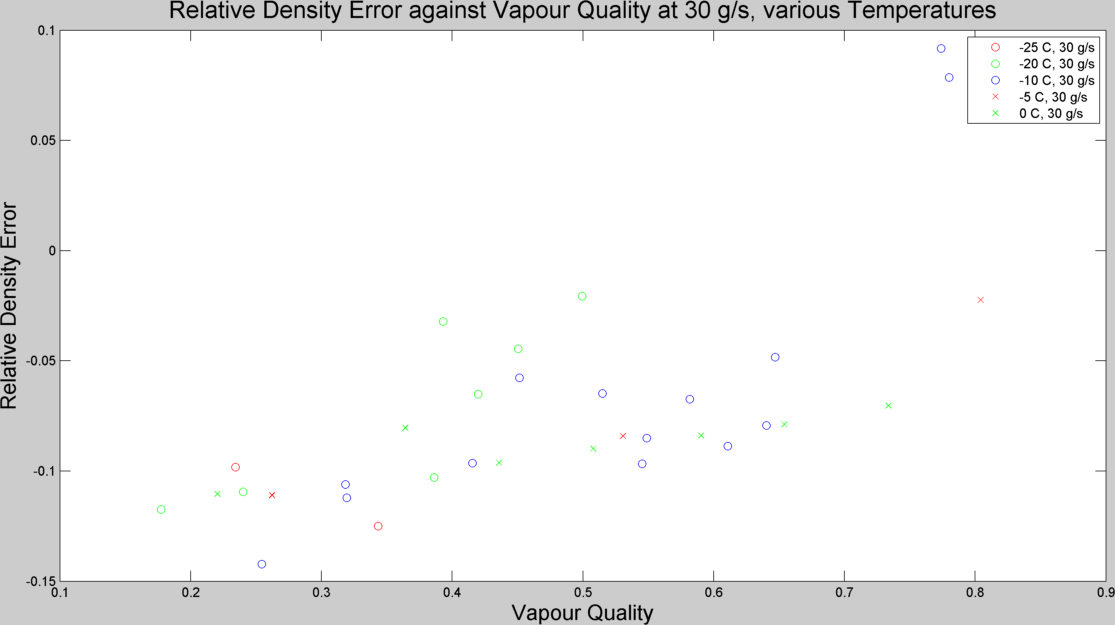
\includegraphics[width=\textwidth]{plots/fig8}
\caption{An overview of relative density error against vapour quality.}
\label{plot:8}
\end{figure}

%VQ ERROR
%30 grams, various temps
\begin{figure}
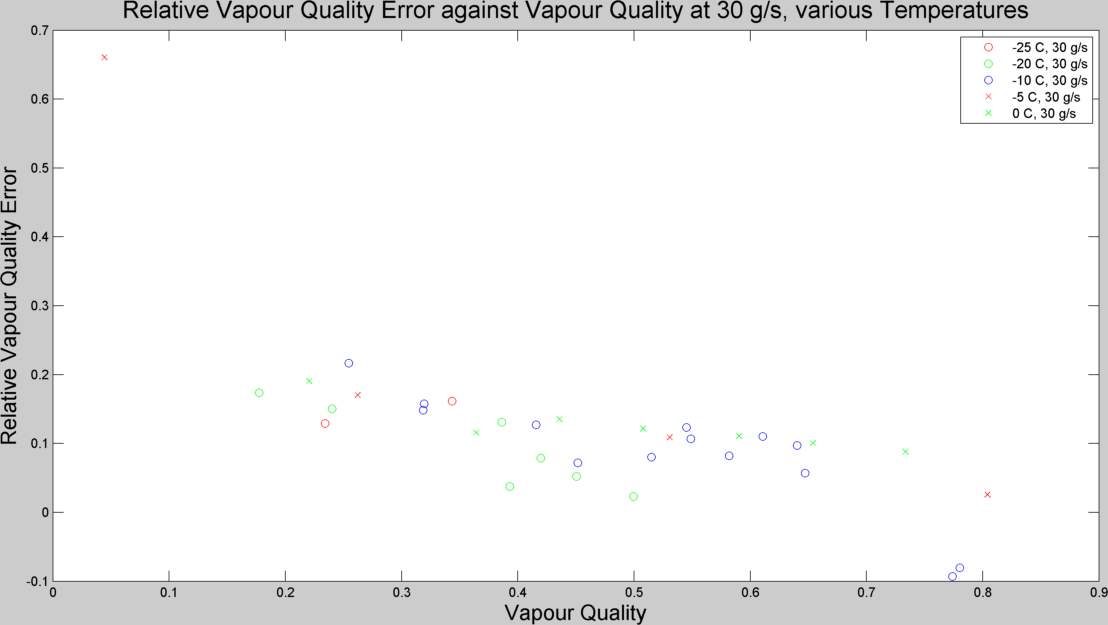
\includegraphics[width=\textwidth]{plots/fig9}
\caption{An overview of relative density error against vapour quality.}
\label{plot:9}
\end{figure}
%20 grams
\begin{figure}
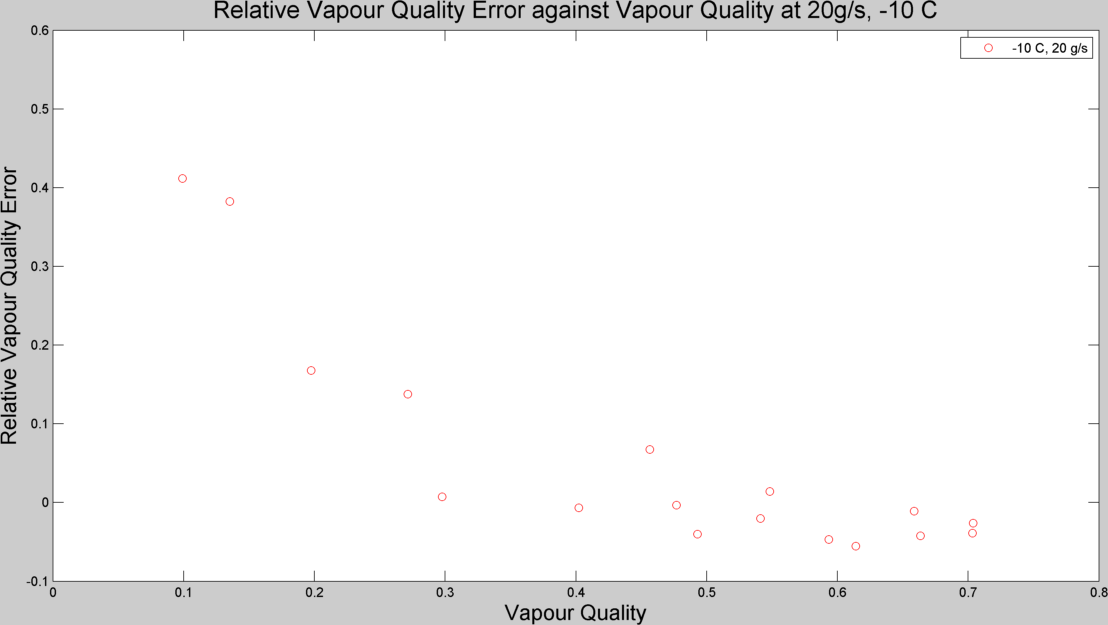
\includegraphics[width=\textwidth]{plots/fig10}
\caption{An overview of relative density error against vapour quality.}
\label{plot:10}
\end{figure}
\chapter{Discussion}

%gas phase flow rate. reduced pressure. undersized instrument. 
\chapter{Conclusions}
\chapter{Future Work}\label{future work}
larger flow meter, dedicated test rig, volumetric flow rate of gas phase? flow regimes, frequency domain analysis, flow meter positioning. real time reference condition calculation. flow velocity. test low flows using bypass. chiller management. definition of true performance envelope.two-phase signal what does it mean?
\iffalse
\bibliographystyle{ieeetr}
\bibliography{bibfile}
\fi
\begin{thebibliography}{9}
\bibitem{O'Banion 2013}
Tom O'Banion,  "Coriolis: the direct approach to mass flow measurement." \textit{Chemical Engineering Progress} 109.3 2013, pp. 41-46.

\bibitem{mastrullo 2010}
R. Mastrullo, A.W. Mauro, A. Rosato, G.P. Vanoli"Carbon dioxide heat transfer coefficients and pressure drops during flow boiling: Assessment of predictive methods." \textit{International Journal of Refrigeration} 2010, vol. 33, pp. 1068-1085

\bibitem{iso}
International Organization for Standardization. "ISO 10790:2015(E) Measurement of fluid in closed conduits - Guidance to the selection, installation and use of Coriolis flowmeters (mass flow, density and volume flow measurements)." 2015

\bibitem{mastrullo 2009a}
R. R. Mastrullo, A.W. Mauro, A. Rosato, G.P. Vanoli. "Carbon dioxide local heat transfer coefficients during flow boiling in a horizontal circular smooth tube." \textit{International Journal of Heat and Mass Transfer} 2009, vol. 52, pp. 4184-4194

\bibitem{TIF PoS}
P. Tropea \textit{et al.} "Design, construction and commissioning of a 15 kW CO$_2$ evaporative cooling system for particle physics detectors: lessons learnt and perspectives for further development" \textit{Proceedings of Science}, 2014, Paper no. 223

\bibitem{jerome} 
J. Daguin \textit{et al.} "Evaporative $CO_2$ Cooling System for the Upgrade of the CMS Pixel Detector at CERN", \textit{10th IIR Gustav Lorentzen Conference on Natural Refrigerants}, 2012, Paper no. 188.
%Krohne http://optimass6400.krohne.com/#introduction

\bibitem{krohne online}
Krohne Group. "Optimass 6400" Internet: \underline{http://optimass6400.krohne.com/\#\_introduction}, [Feb. 18, 2015]

\bibitem{krohne brochure}
Krohne Group. "Optimass 6400." Brochure. Apr 2013

\bibitem{thome 1}
L. Cheng, G. Ribatski, J. M. Quib$\acute{e}$n, J R. Thome. "New prediction methods for CO$_2$ evaporation inside tubes: Part I - A two-phase flow pattern map and a flow pattern based phenomenological model for two-phase flow frictional pressure drops." \textit{International Journal of Heat and Mass Transfer} vol. 51, pp. 111-124, 2008

\bibitem{bart}
B. Verlaat. "Controlling a 2-phase CO2 loop using a 2-phase accumulator." \textit{International Conference of Refrigeration}, 2007, Beijing, China, ICR07-B2-1565 

\bibitem{bart2}
A.P. Colijn, B. Verlaat. "Evaporative CO$_2$ Heat Transfer Measurements for Cooling Systems of Partical Physics Detectors." \textit{7$^{
th}$ International Conference on Heat Transfer, Fluid Mechanics and Thermodynamics}, 2010, Antalaya, Turkey, HEFAT2010 

\bibitem{mishra}
B. Mishra. "CO$_2$ based two phase cooling test set up for CMS trackers: Comparison of experiments with theoretical models." \textit{CERN CMS Collaboration}

\bibitem{CO2 PoS}
B. Verlaat. "CO2 Cooling Developments for HEP Detectors." \textit{Proceedings of Science}, 2009

\bibitem{emerson youtube}
Emerson Electric Co. Video File: "Demonstration: Coriolis Flowmeter excels with Two-Phase Flow (entrained gas)." Retrieved from \underline{https://www.youtube.com/watch?v=AjtdNxDOeoo}, Jan. 17, 2013, [Mar. 15, 2015]

\bibitem{tif web}
P. Tropea. "The CMS PIX Phase I upgrade CO2 cooling: a full scale prototype ready for tests." Internet: \underline{http://ph-news.web.cern.ch/content/cms-pix-phase-i-upgrade-co2-cooling-full-scale-prototype-ready-tests}, Dec. 13, 2013 [Mar. 14, 2015] 

\bibitem{emerson EGM}
D. Wehrs, A. Klosinski. "Entrained Gas Diagnostic with Intelligent Differential Pressure Transmitter." White Paper: \textit{Emerson Process Management}, Jan. 2008, p. 1

\bibitem{processArticle}
K. Parker. "Bent-tube Coriolis flowmeter slated for entrained gas, high-temp applications." \textit{Processing Magazine} (Jul. 1, 2013)

\bibitem{CERN courier}
B. Verlaat, "CO2 cooling is getting hot in high-energy physics." \textit{CERN Courier} (May 31, 2012)

\bibitem{Augyrond 2001}
L. Augyrond \textit{et al.} "Void Fraction Measurement in Two-Phse Helium Flow with Electron Energy Attenuation Detector." \textit{Cryogenic Engineering Conference}, Jul. 2001, Madison, WI, USA C-09B-02

\bibitem{Zhao 2013}
Y. Zhao, Q. Bi, R. Hu. "Recognition and measurement in theflow pattern and void fraction of gas-liquid two-phase flow in vertical upward pipes using the gamma densitometer." Applied Thermal Engineering 60 (2013) 398e41

\bibitem{Bauer 2012}
D. Bauer, H. Chaves, and C. Arcoumanis. "Measurements of void fraction distribution in cavitating pipe flow
using x-ray CT." Measurement Science and Technology, Issue 23, 2012

\bibitem{Beker 2005}
M. Beker. "Capacitive measurement technique for void fraction measurements in two phase pipe flow." BSc Project, Delft University of Science and Technology, Delft, the Netherlands, Jul. 2005

\bibitem{lecture}
J. M. Doster, "Flow Regime Mapping, Void-Quality Relations and Pressure Drop in Two Phase Flow." Lecture Notes. Nuclear Engineering Department, North Carolina State University 

\bibitem{Jean 2007}
B. R. Jean. "A Microwave Sensor for Steam Quality." IEEE Transaction on Instrumentation and Measurement, Aug. 2007

\bibitem{Dorfman 2006}
A. Dorfman, E. Fridman. "Vapor quality measurement by a discharging calorimeter." Fluid Phase Equilibria, 244 (2006) 46–51

\end{thebibliography}
\appendix
\chapter{The TIF Cooling System}\label{app:TIF}
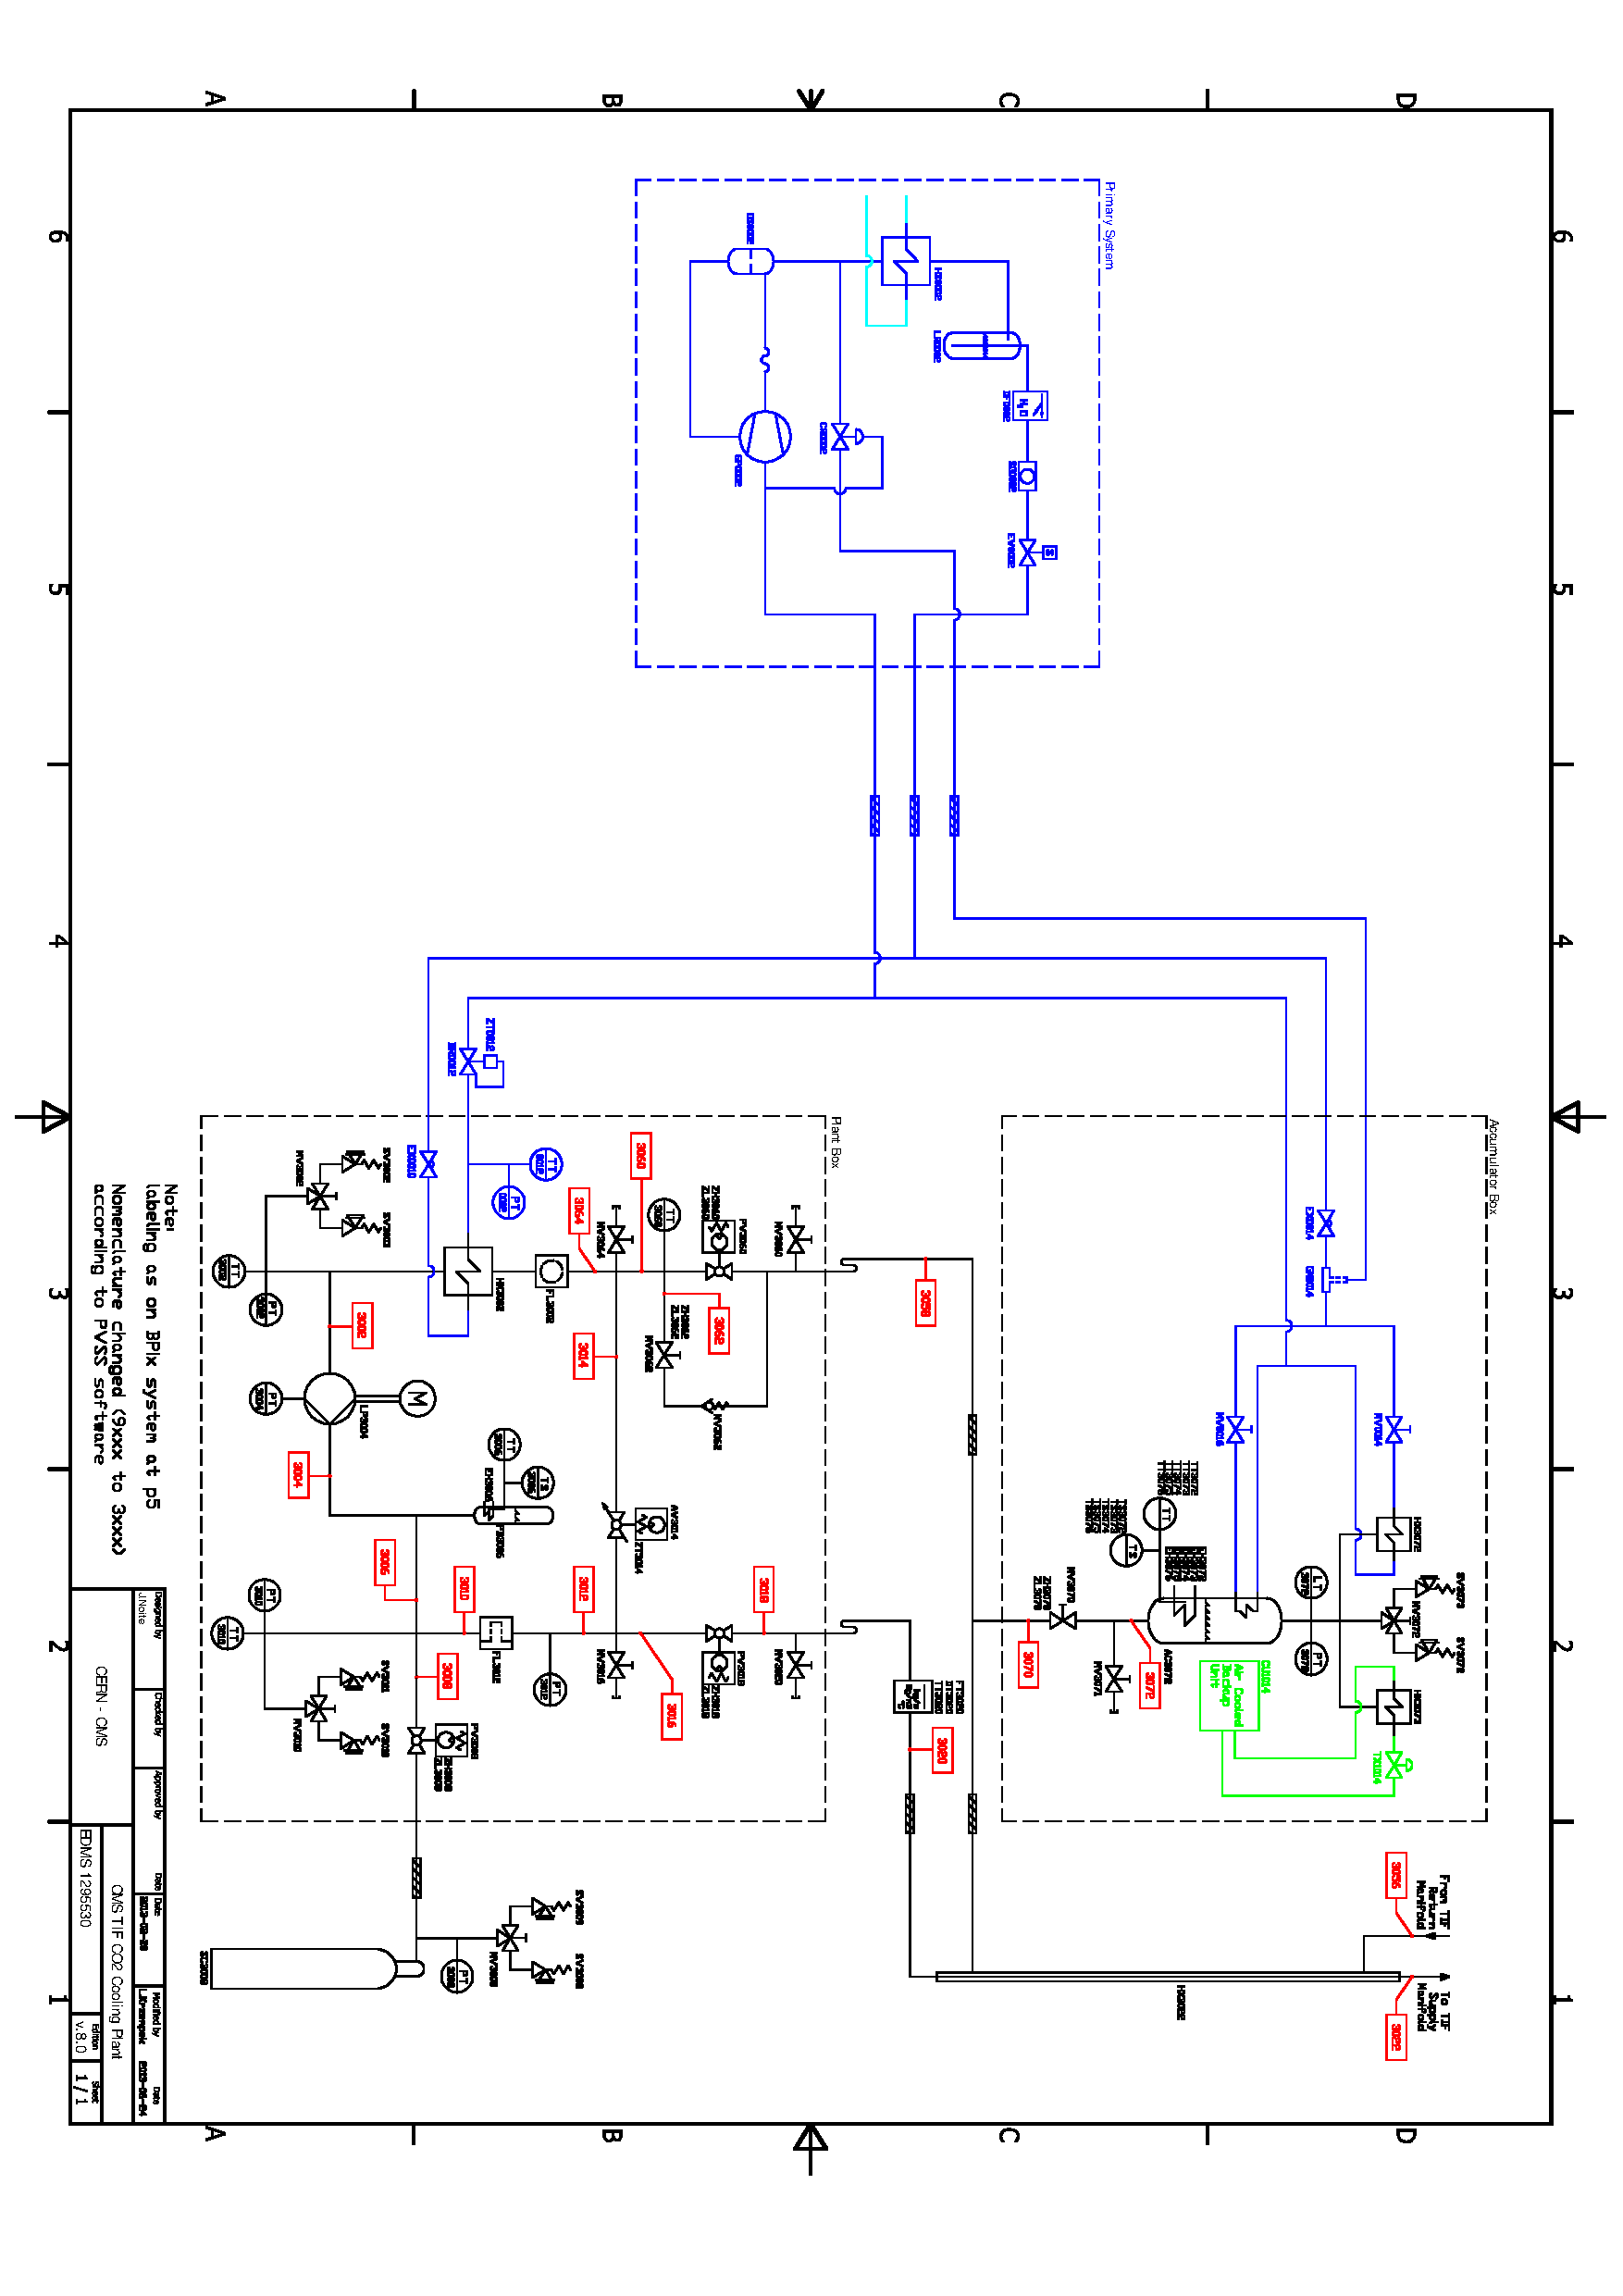
\includepdf{../docs/PI_TIF_Plant.pdf}
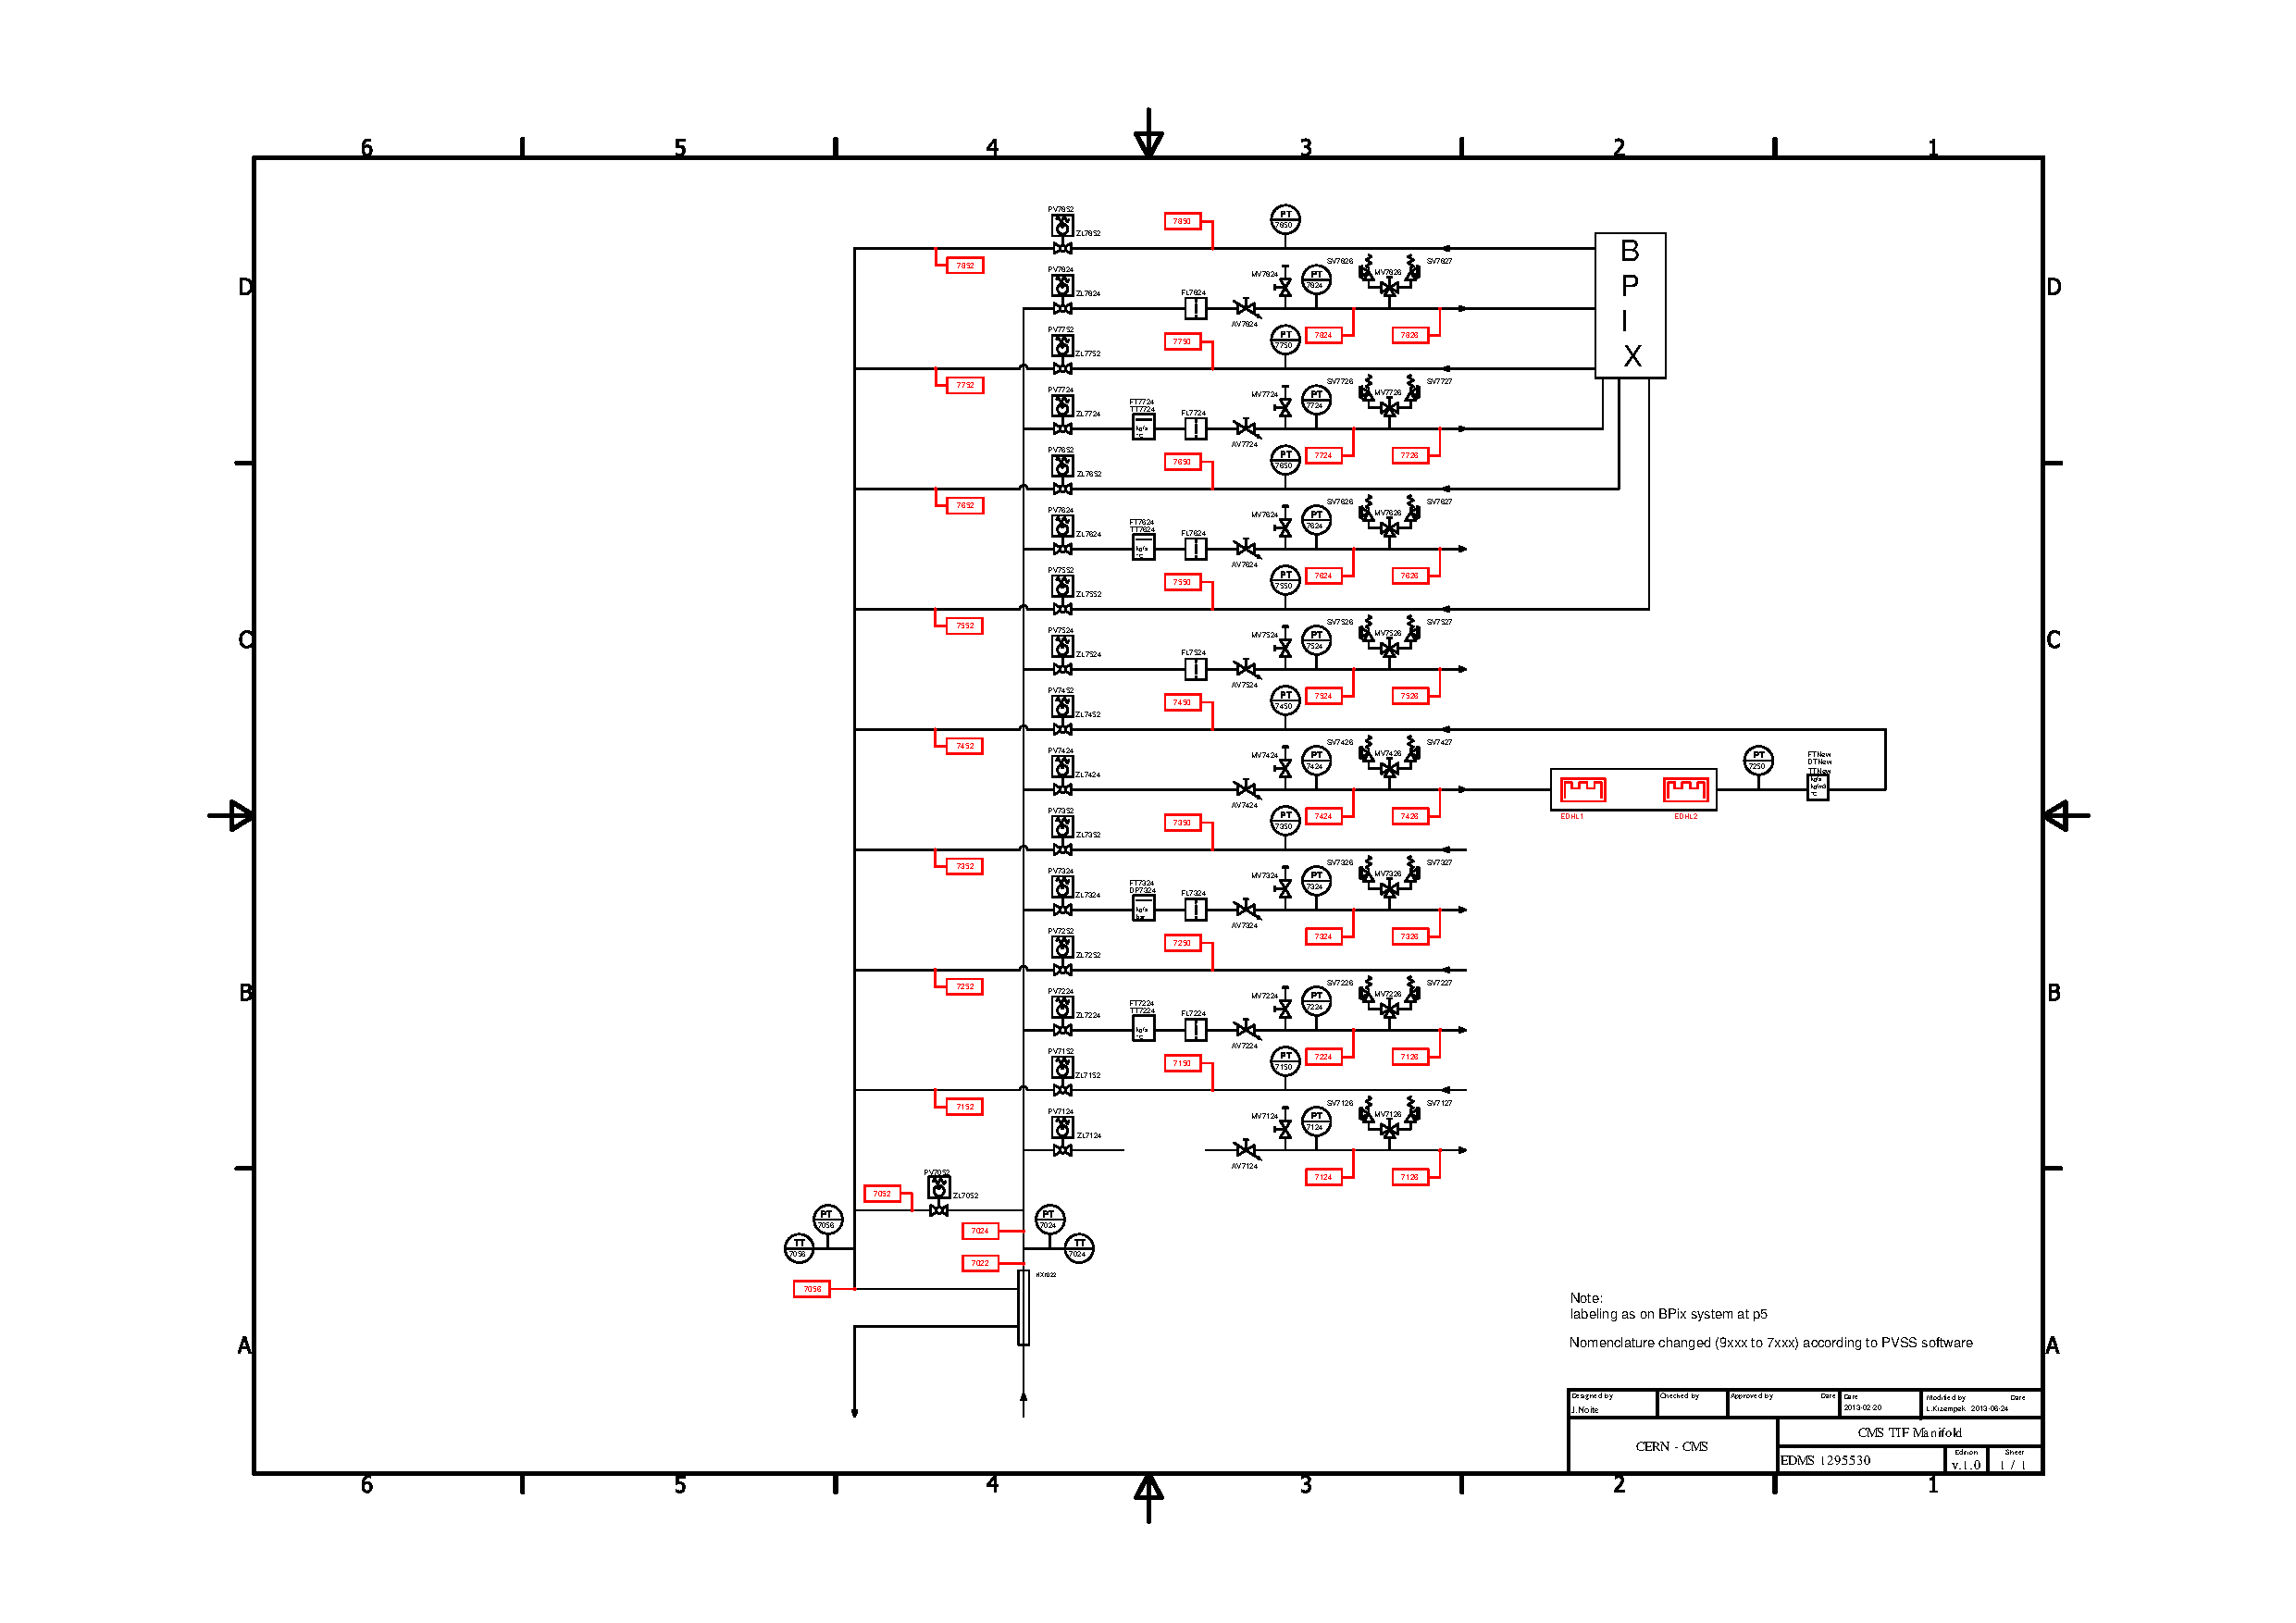
\includepdf[landscape]{../docs/PI_TIF_Manifold.pdf}
\chapter{Krohne Calibration and Sizing Documents}
%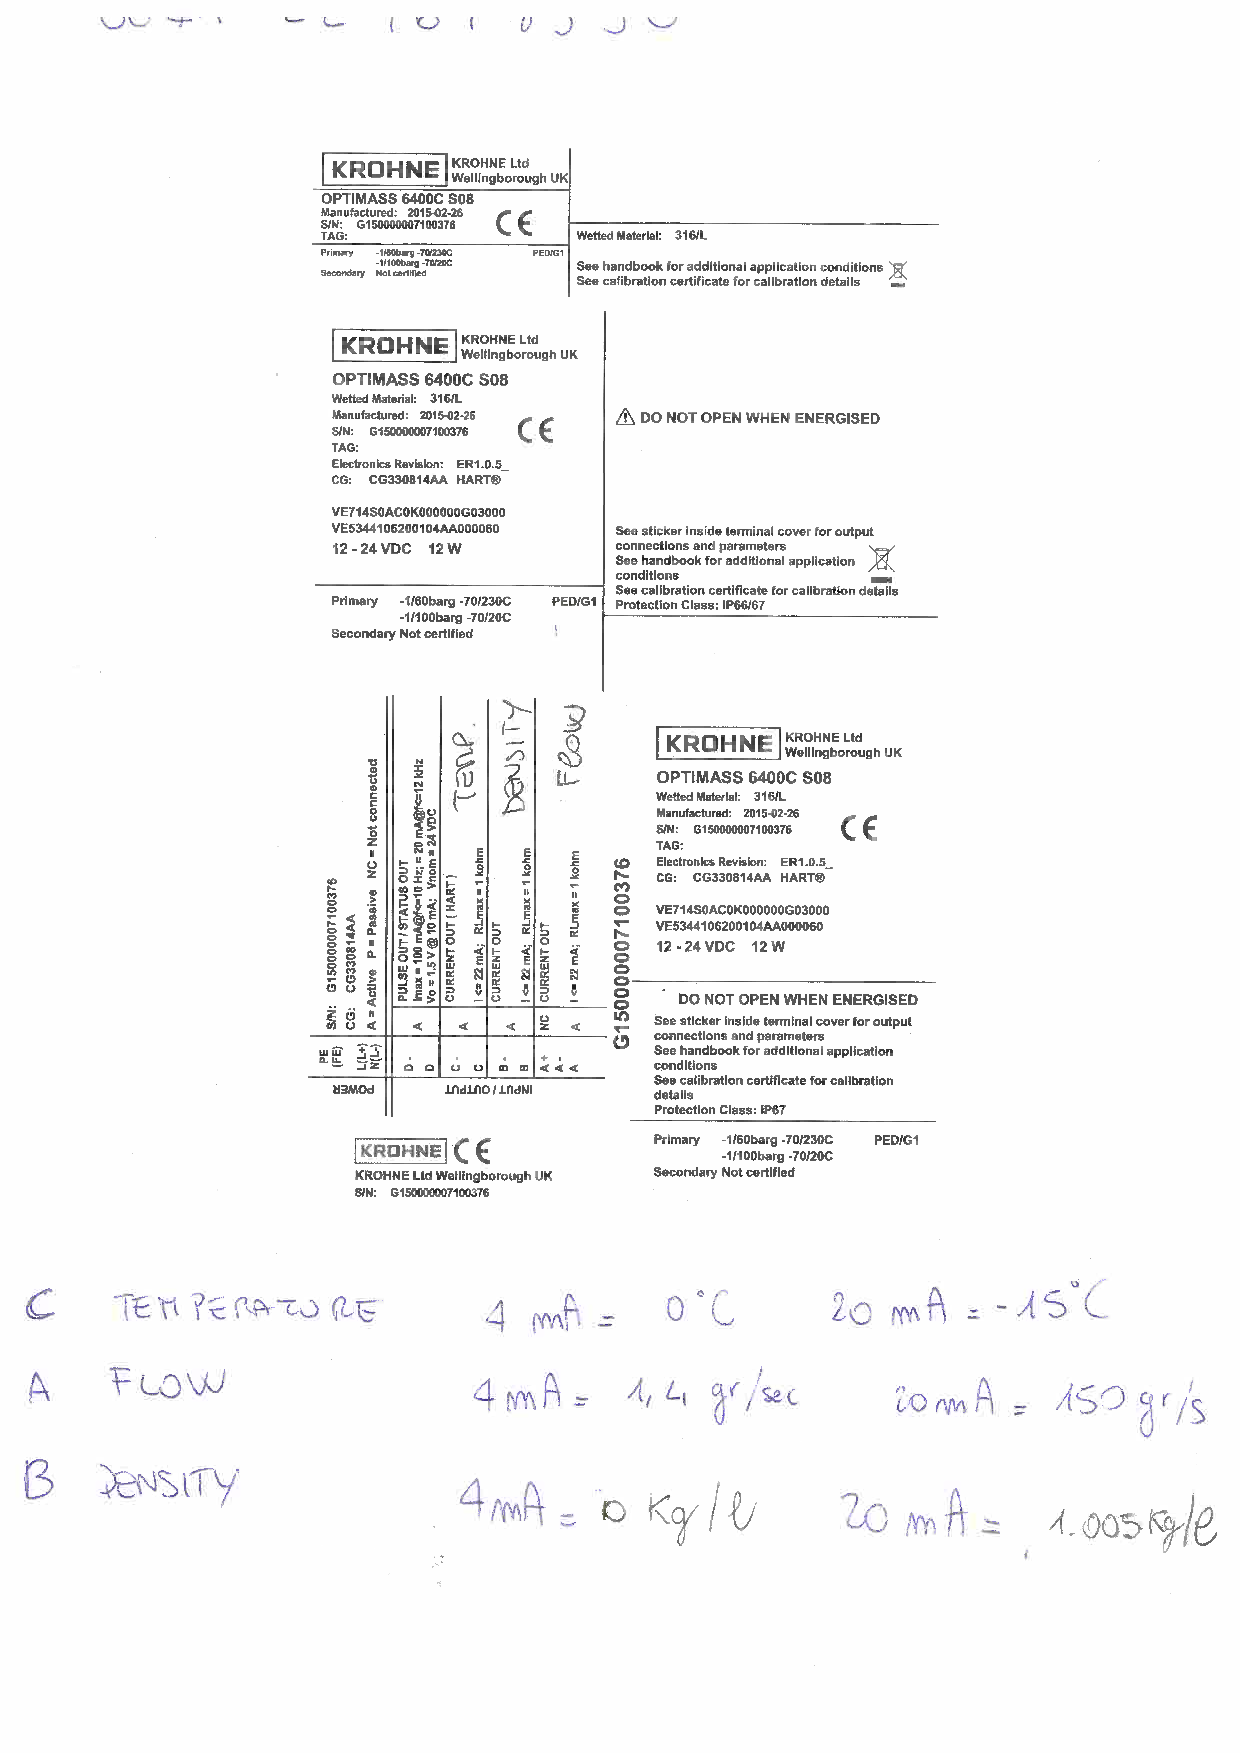
\includepdf{../docs/calibration.pdf}
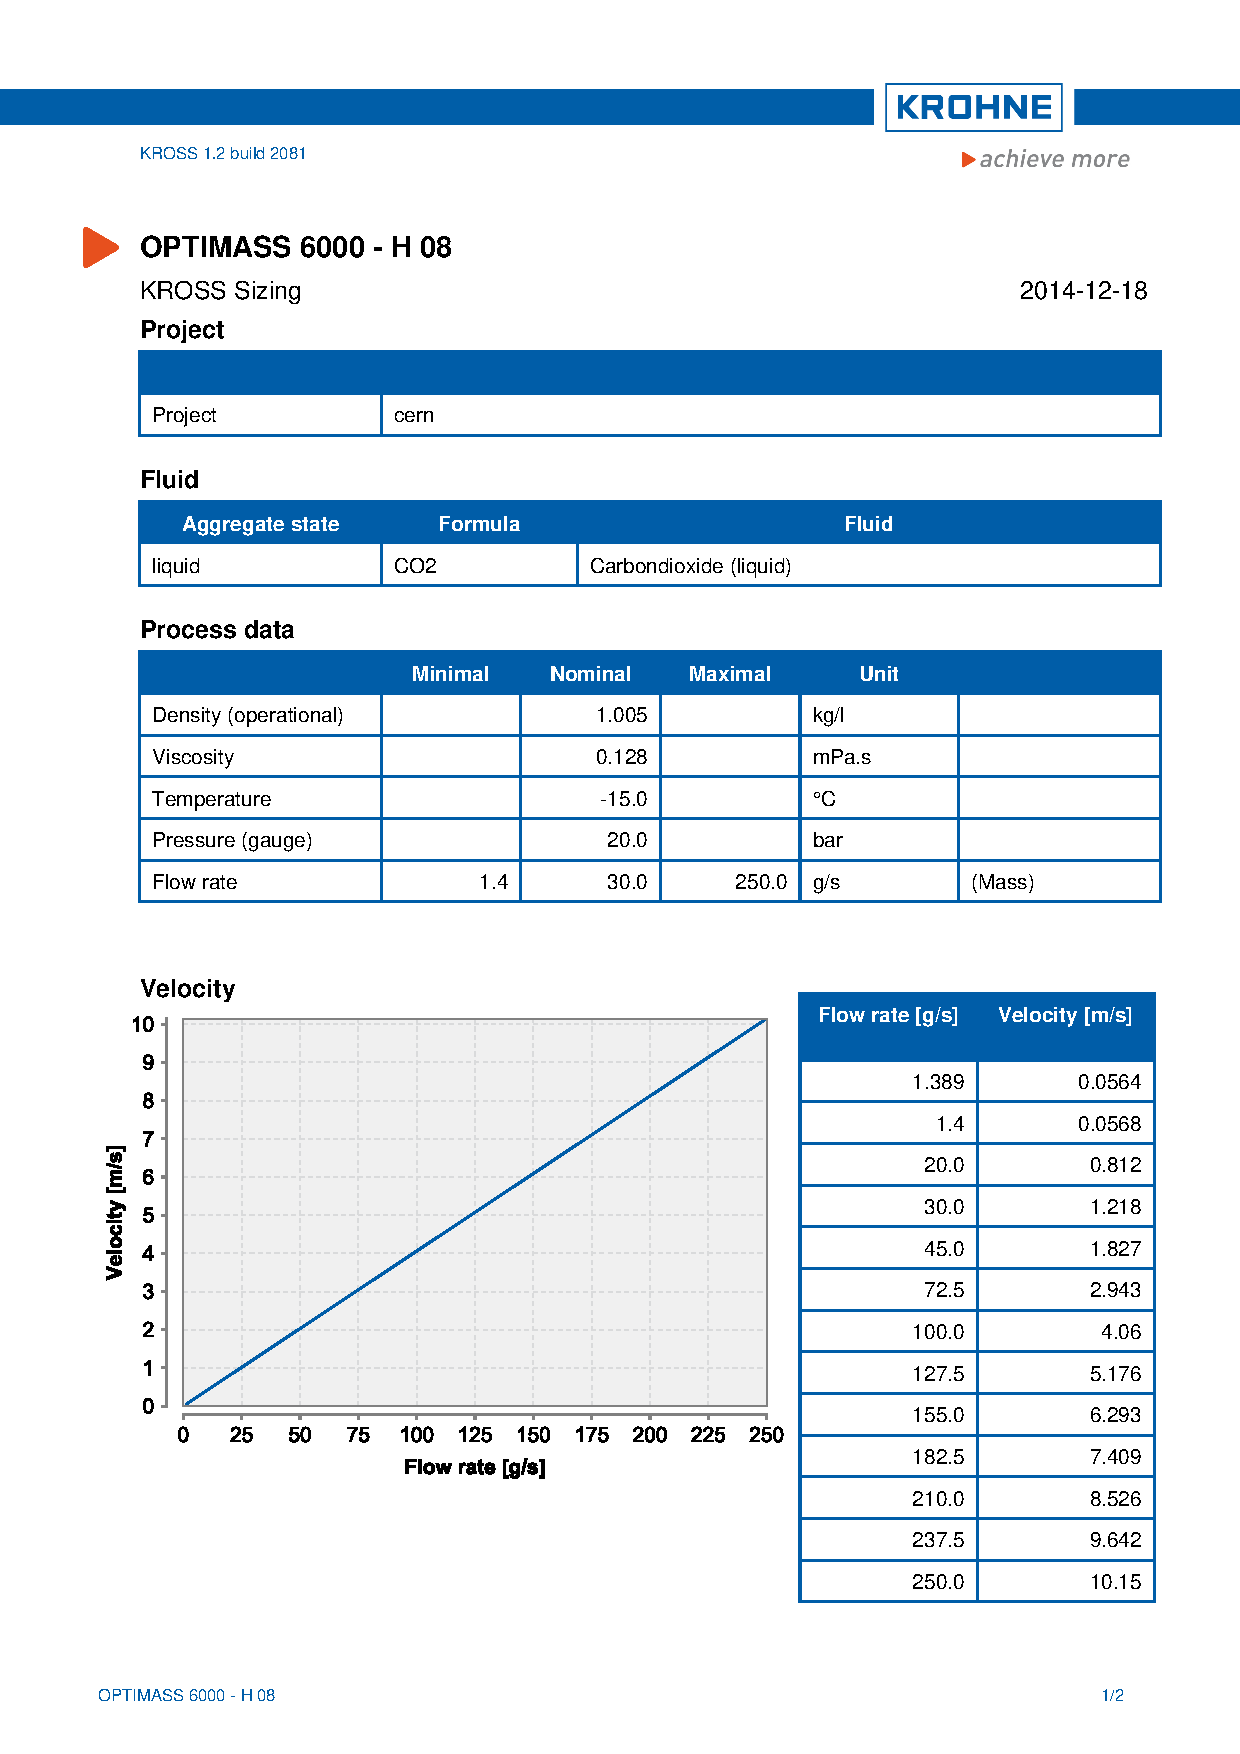
\includepdf{../docs/sizing.pdf}


\chapter{Dummy Load Heater Module Mechanical Design} \label{app:DummyLoad}
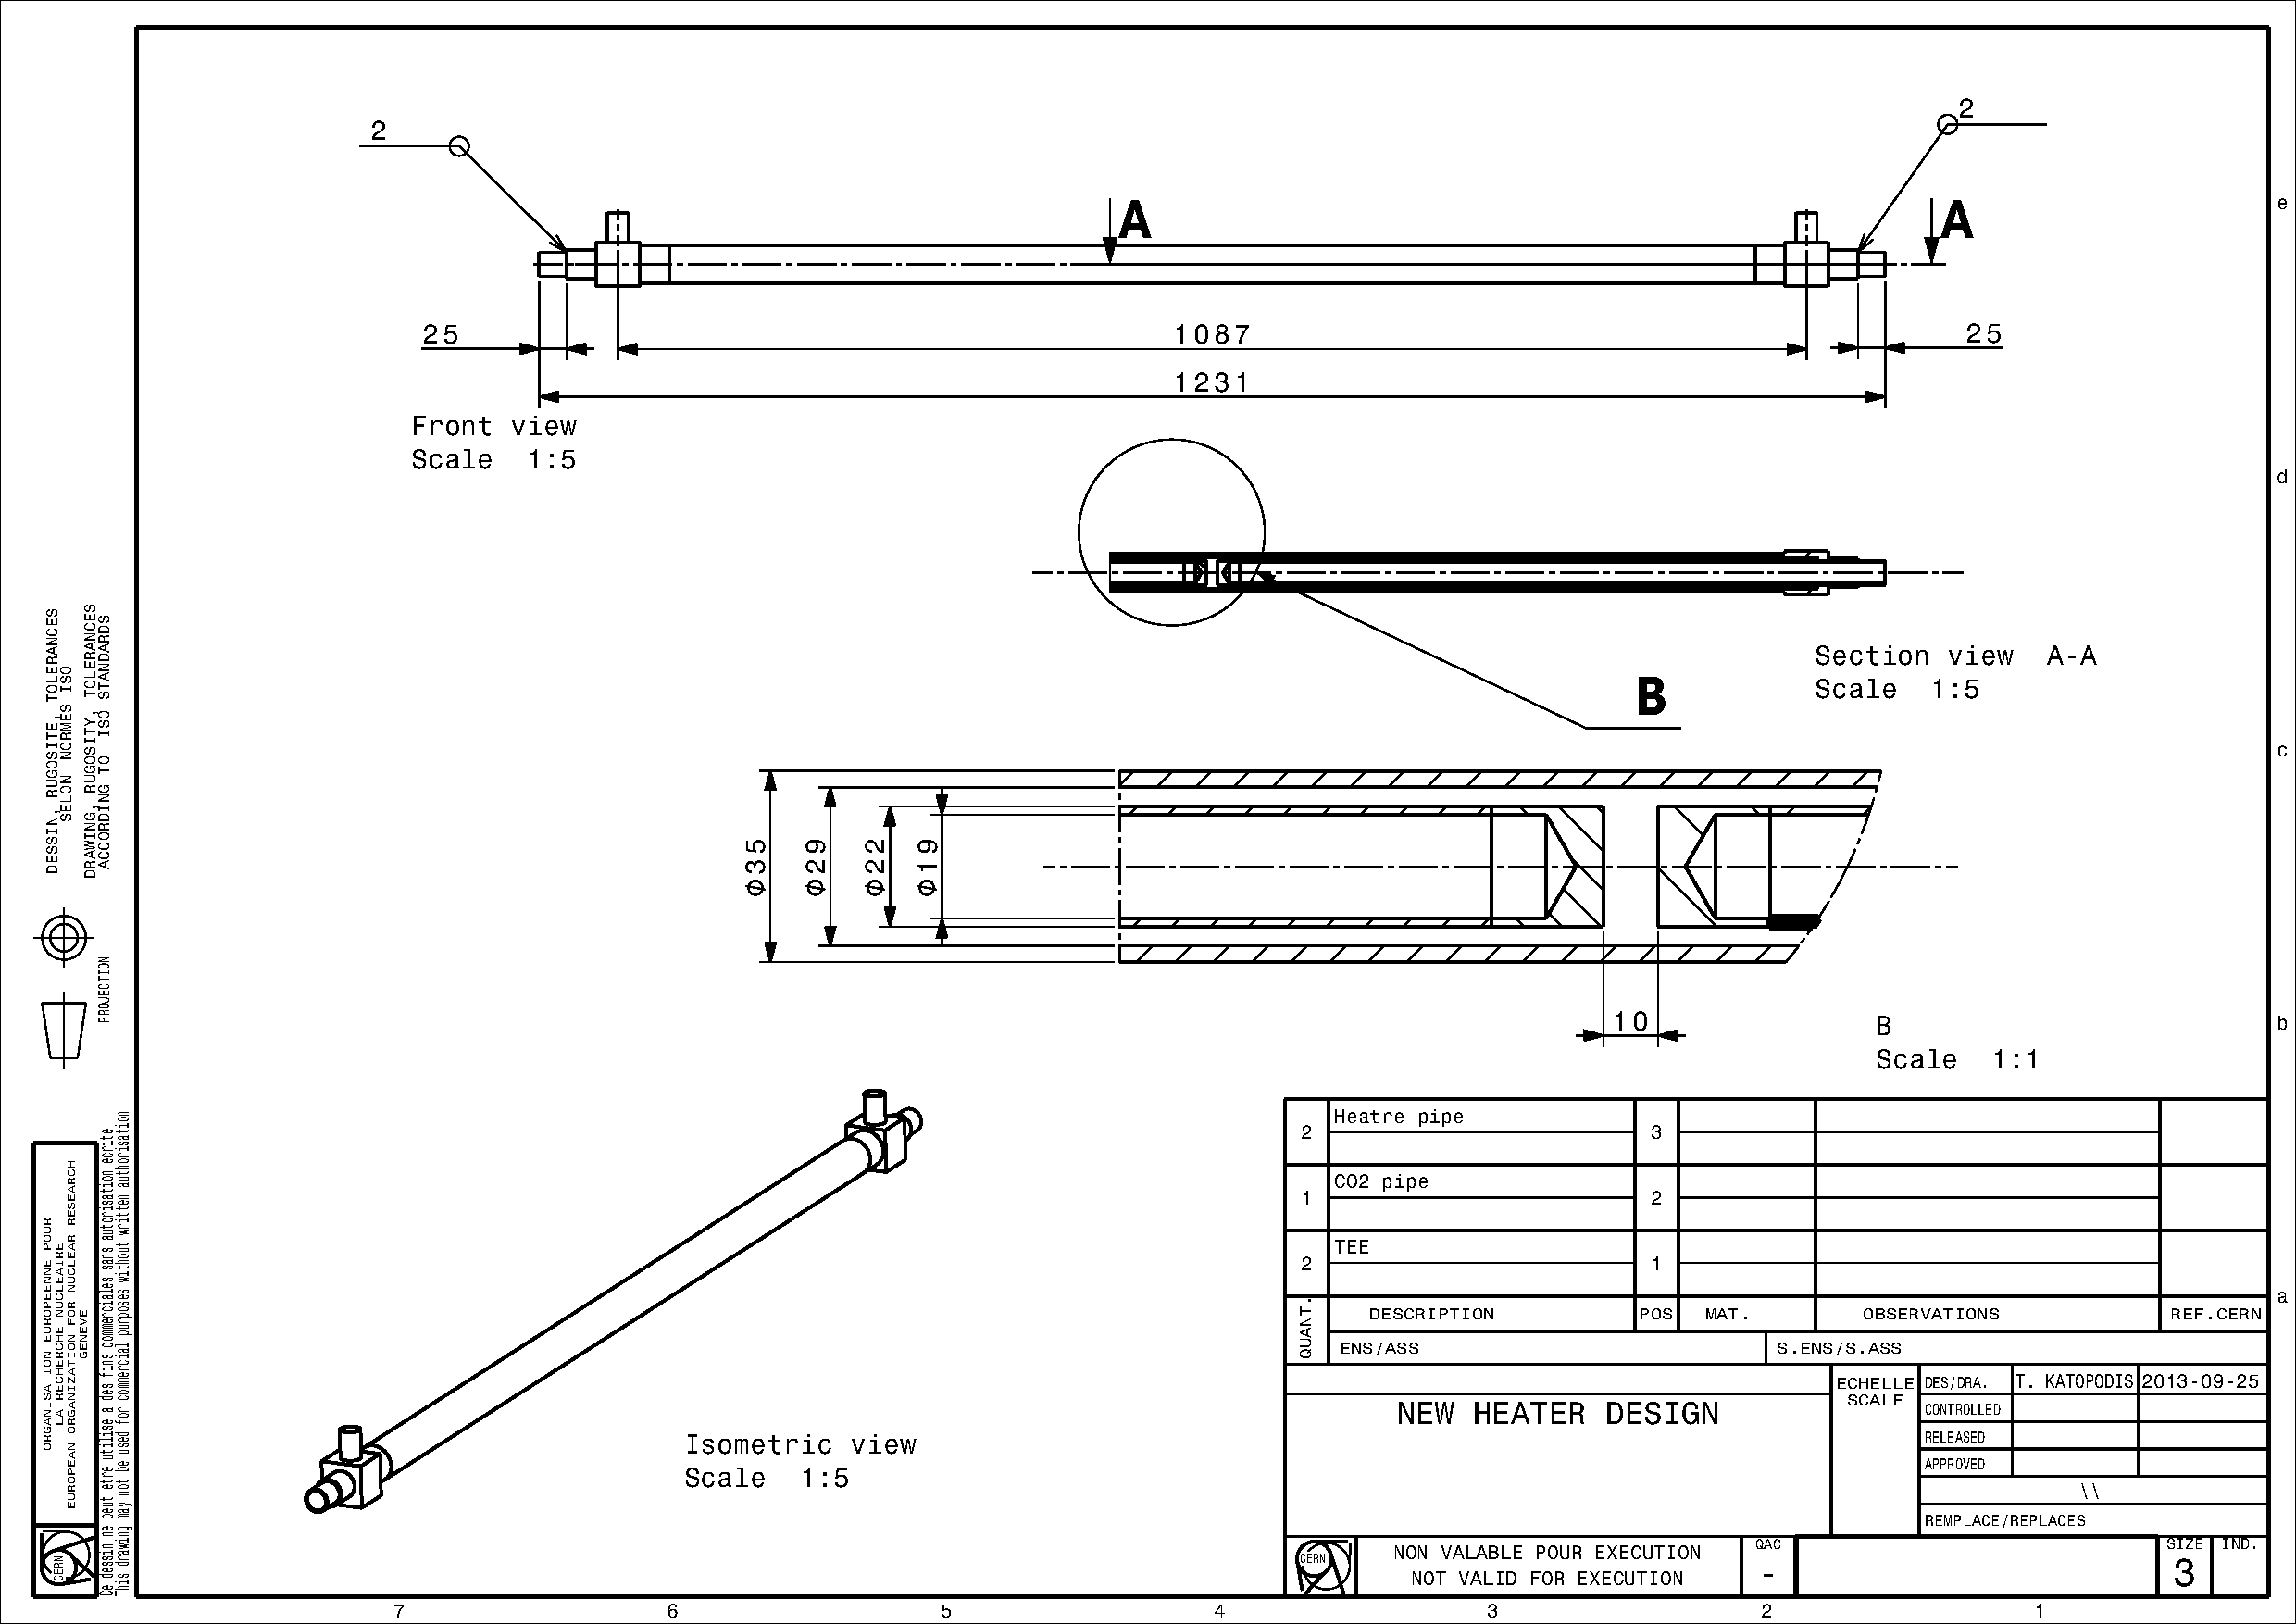
\includepdf[landscape]{../docs/Heater_Design.pdf}
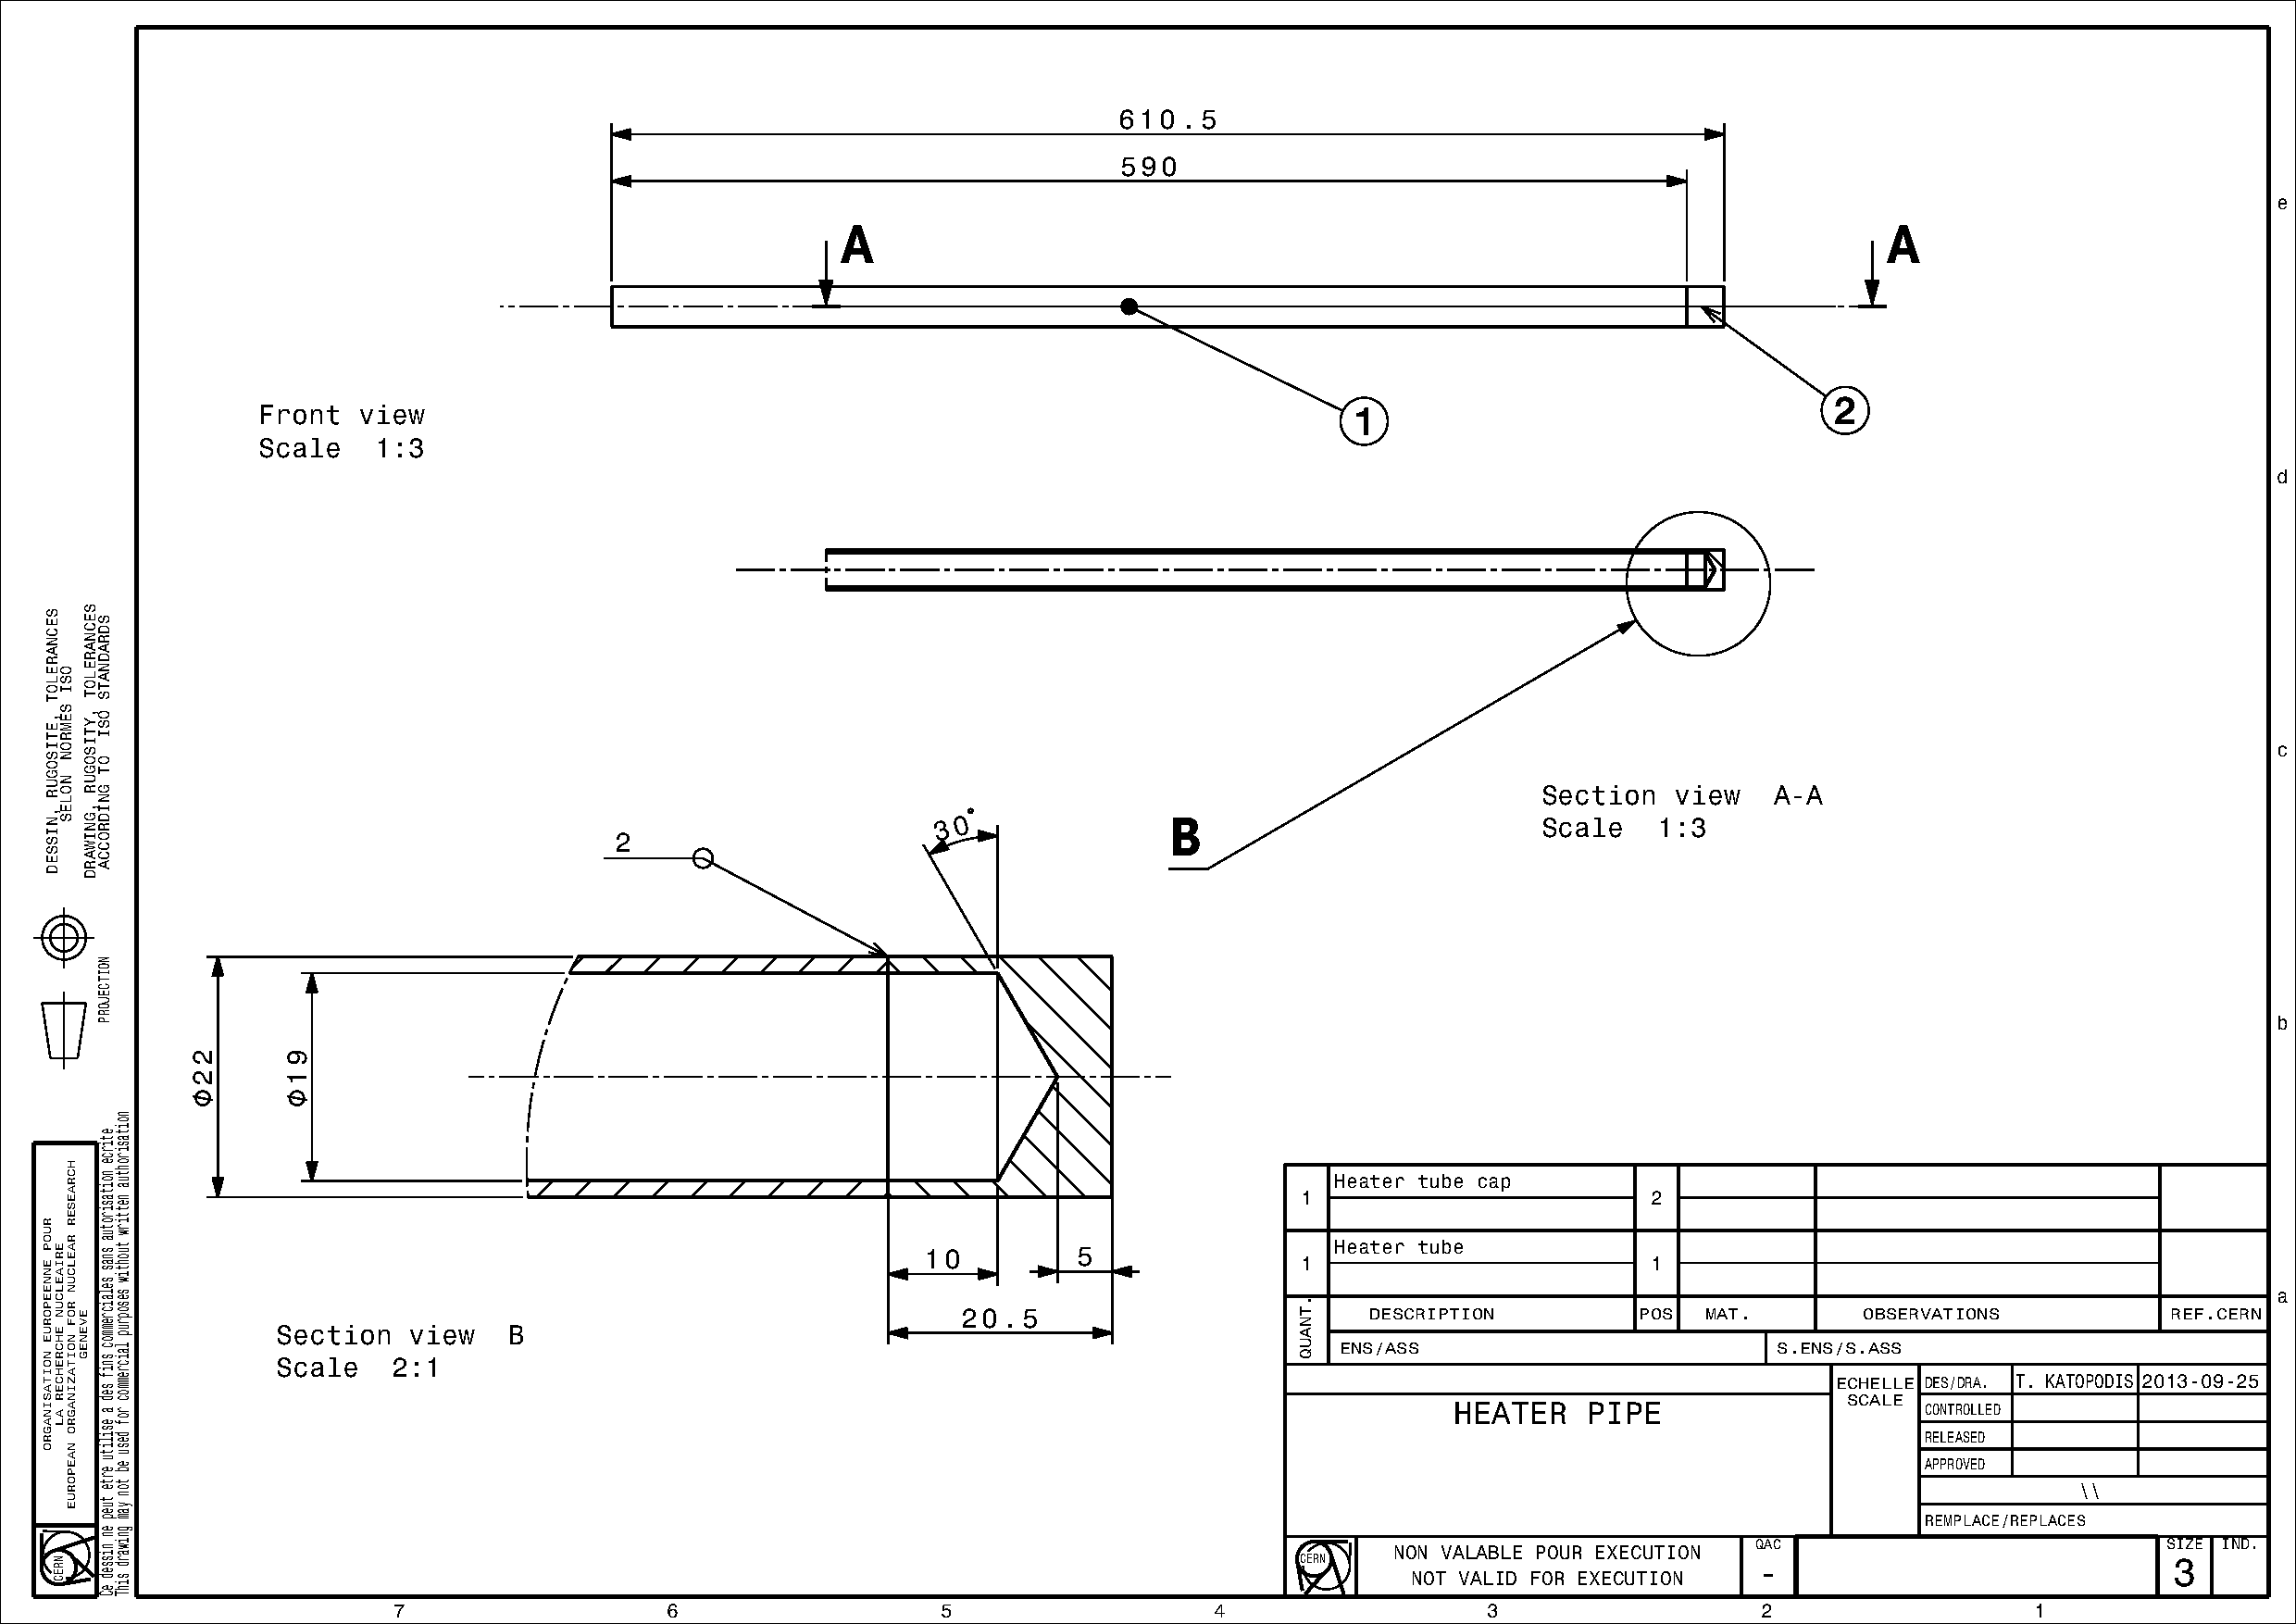
\includepdf[landscape]{../docs/heater2.pdf}
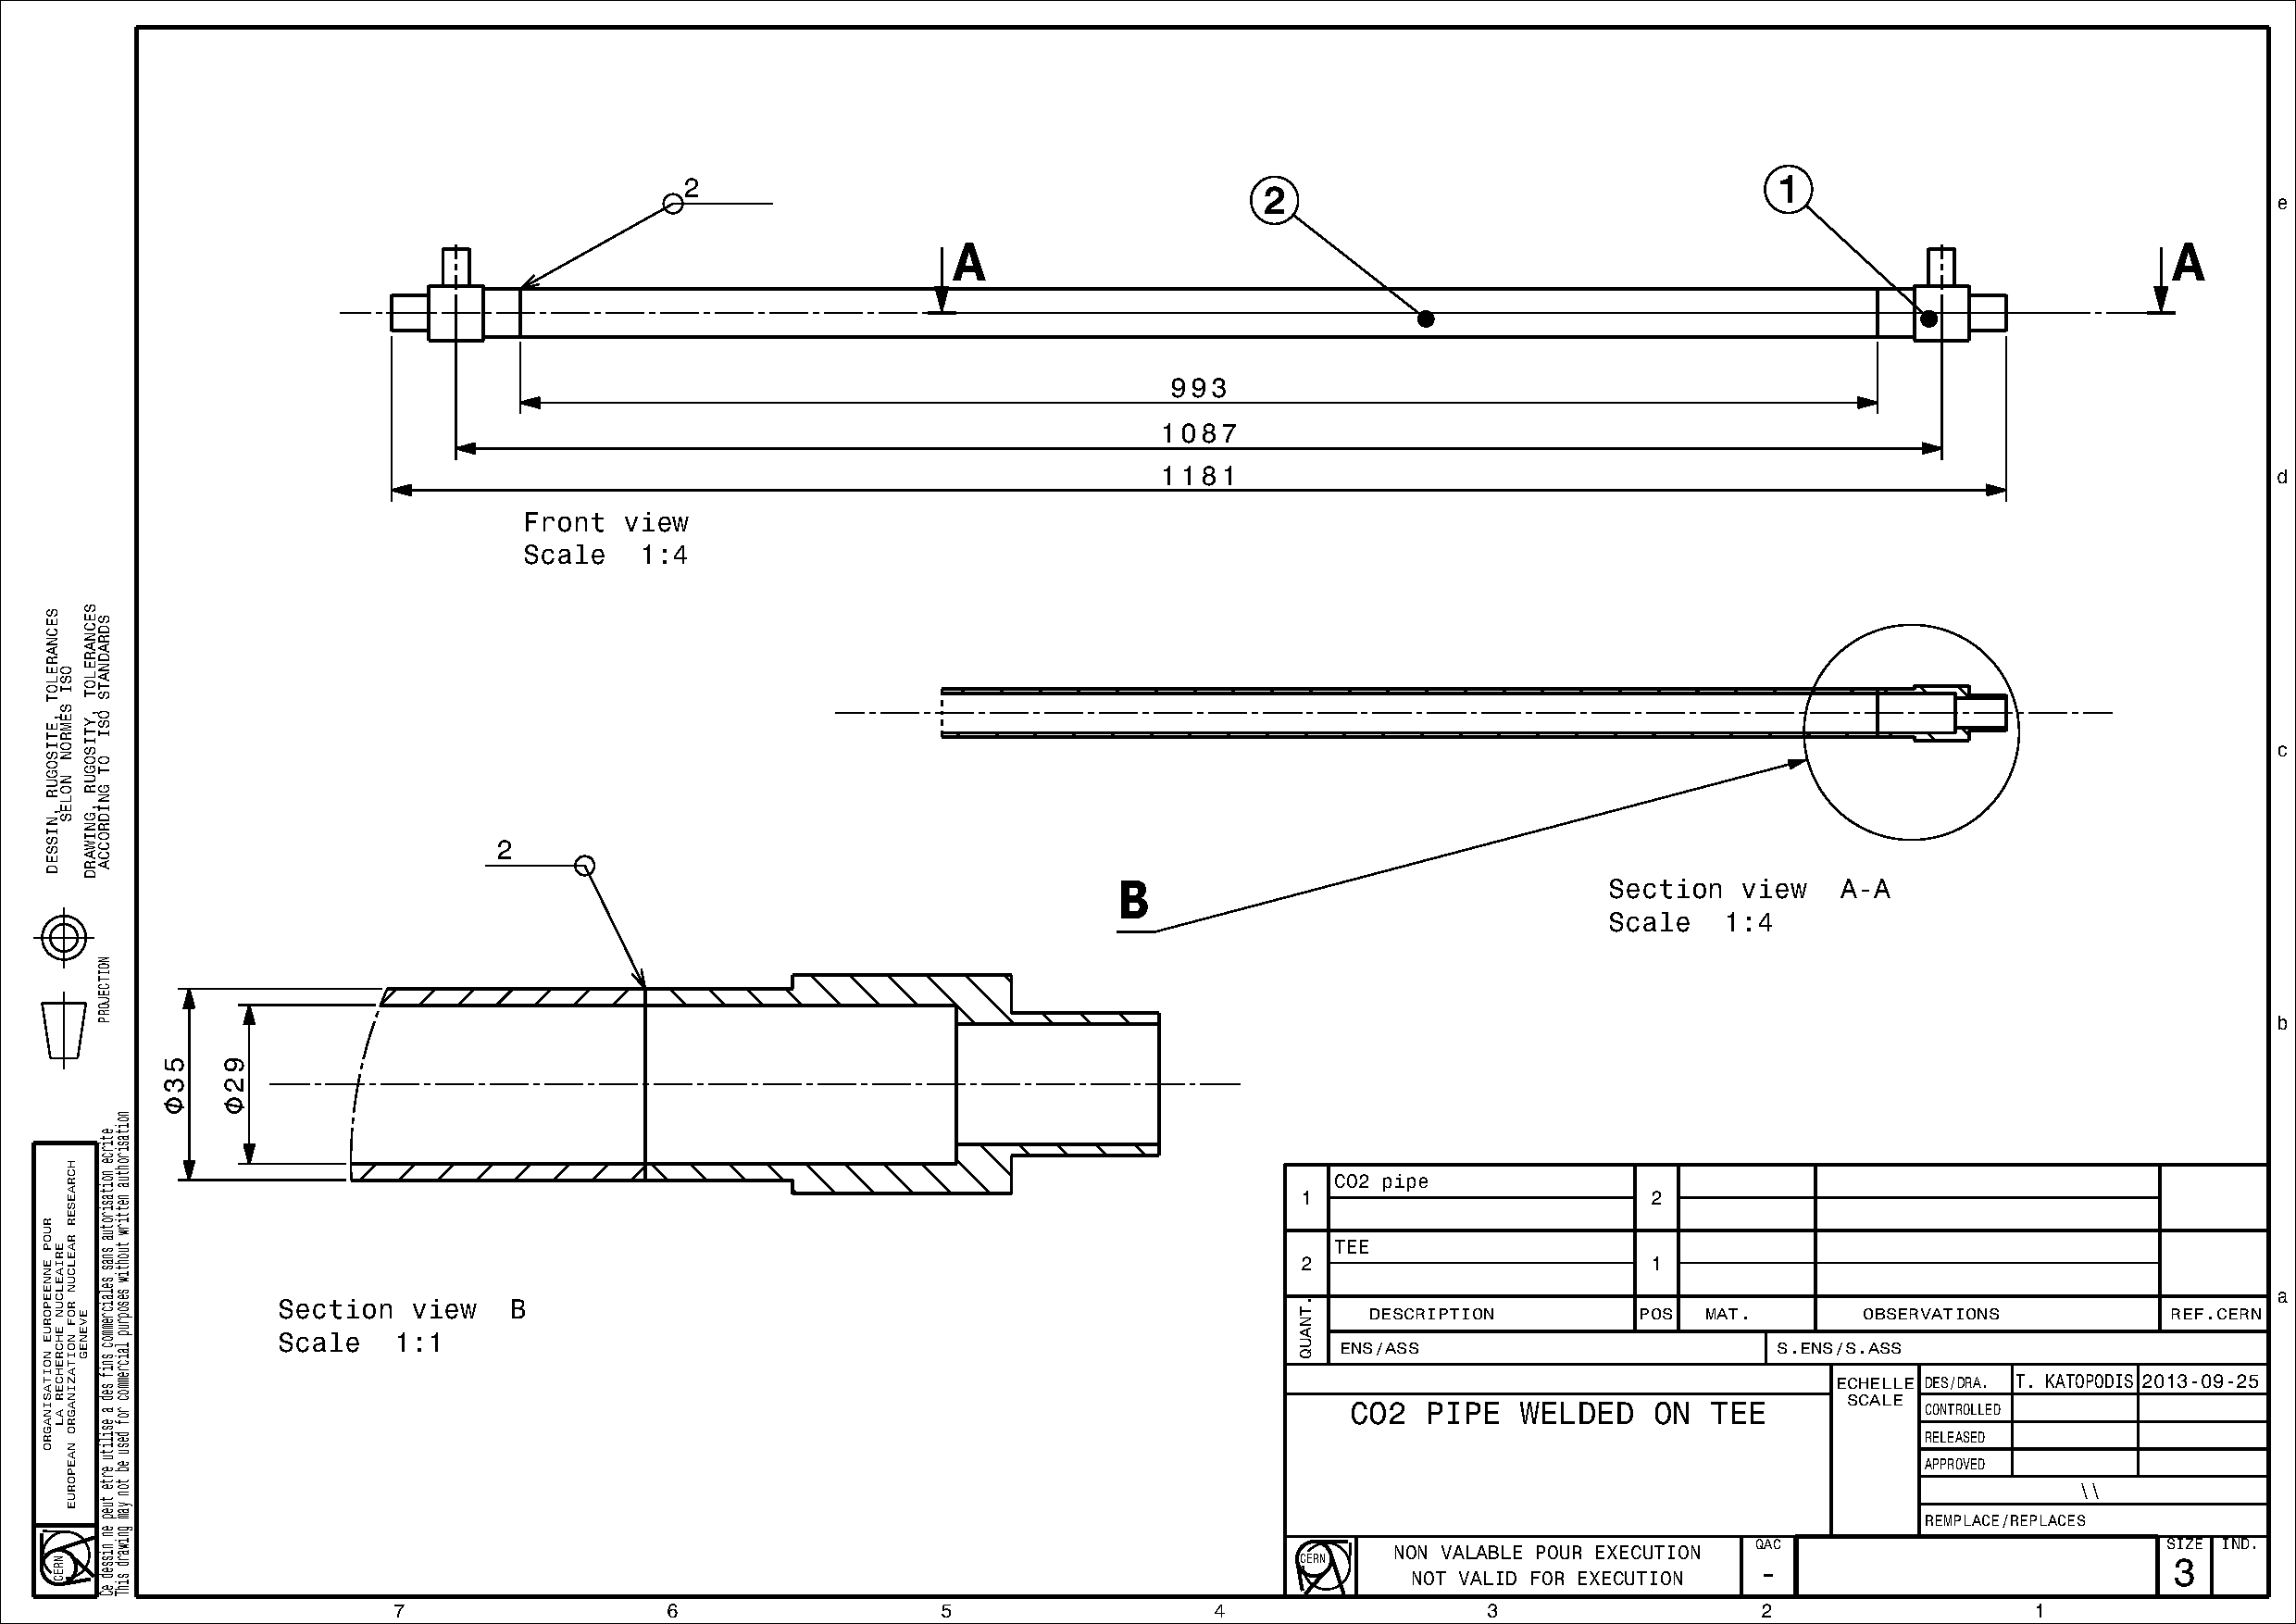
\includepdf[landscape]{../docs/heater3.pdf}
\chapter{MATLAB Code}
\chapter{Raw Data}
\end{document}
